\documentclass{article}
\usepackage[utf8]{inputenc}
\usepackage[top=1.25in, bottom=1.25in, left=1.5in, right=1.5in]{geometry}
\usepackage{graphicx}

\title{\vspace{5cm}\textbf{Mesa Interactiva BarISTa}\\Manual de Utilizador}

\begin{document}
\maketitle
\newpage

\tableofcontents
\newpage

\section{Ecrã Principal}
Quando o utilizador entra no Barista depara-se com o seguinte ecrã:\\
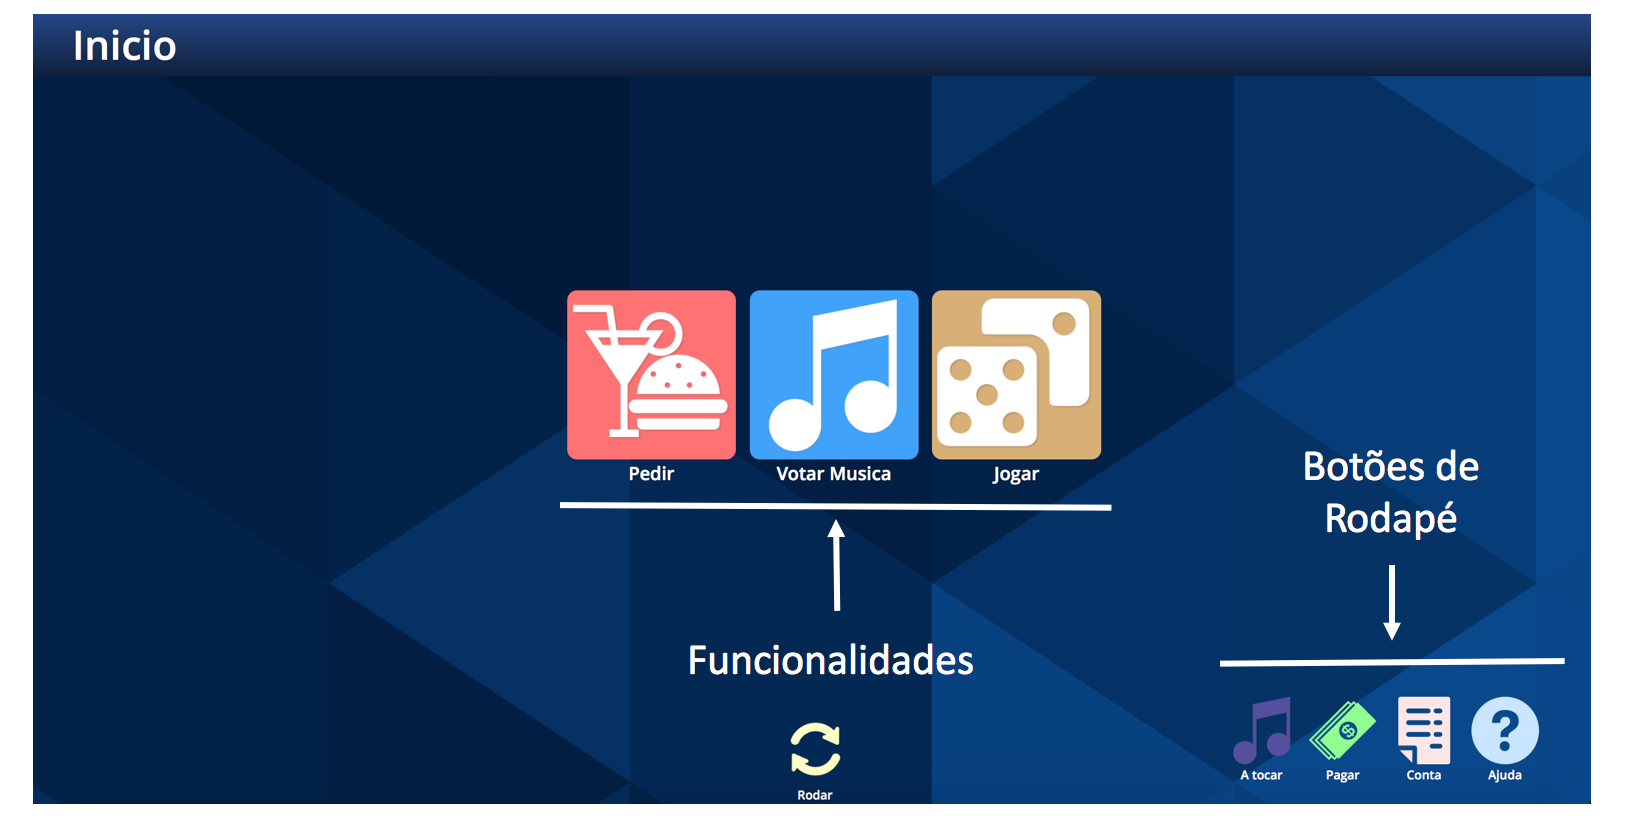
\includegraphics[width=15cm, height=8cm]{user_manual_images/chick.png}
O utilizador poderá clicar em qualquer uma das funcionalidades que pretende aceder, sendo que existem três:
\begin{itemize} 
\item Pedir (onde pode pedir bebidas, snacks e criar o seu próprio cocktail)
\item Votar Música  (onde pode votar na música que deseja ouvir)
\item Jogar 
\end{itemize}
No rodapé é possível observar 4 botões:
\begin{itemize} 
\item A tocar (mostra a música que está a tocar e a próxima na playlist)
\item Pagar   (leva o utilizador ao ecrã de pagamento)
\item Conta   (mostra tudo o que o utilizador já pediu - conta)
\item Ajuda   (apresenta uma explicação de cada ecrã)
\end{itemize}
Os botões de rodapé estão presentes em todos os ecrãs da aplicação.
\section{Pedidos}
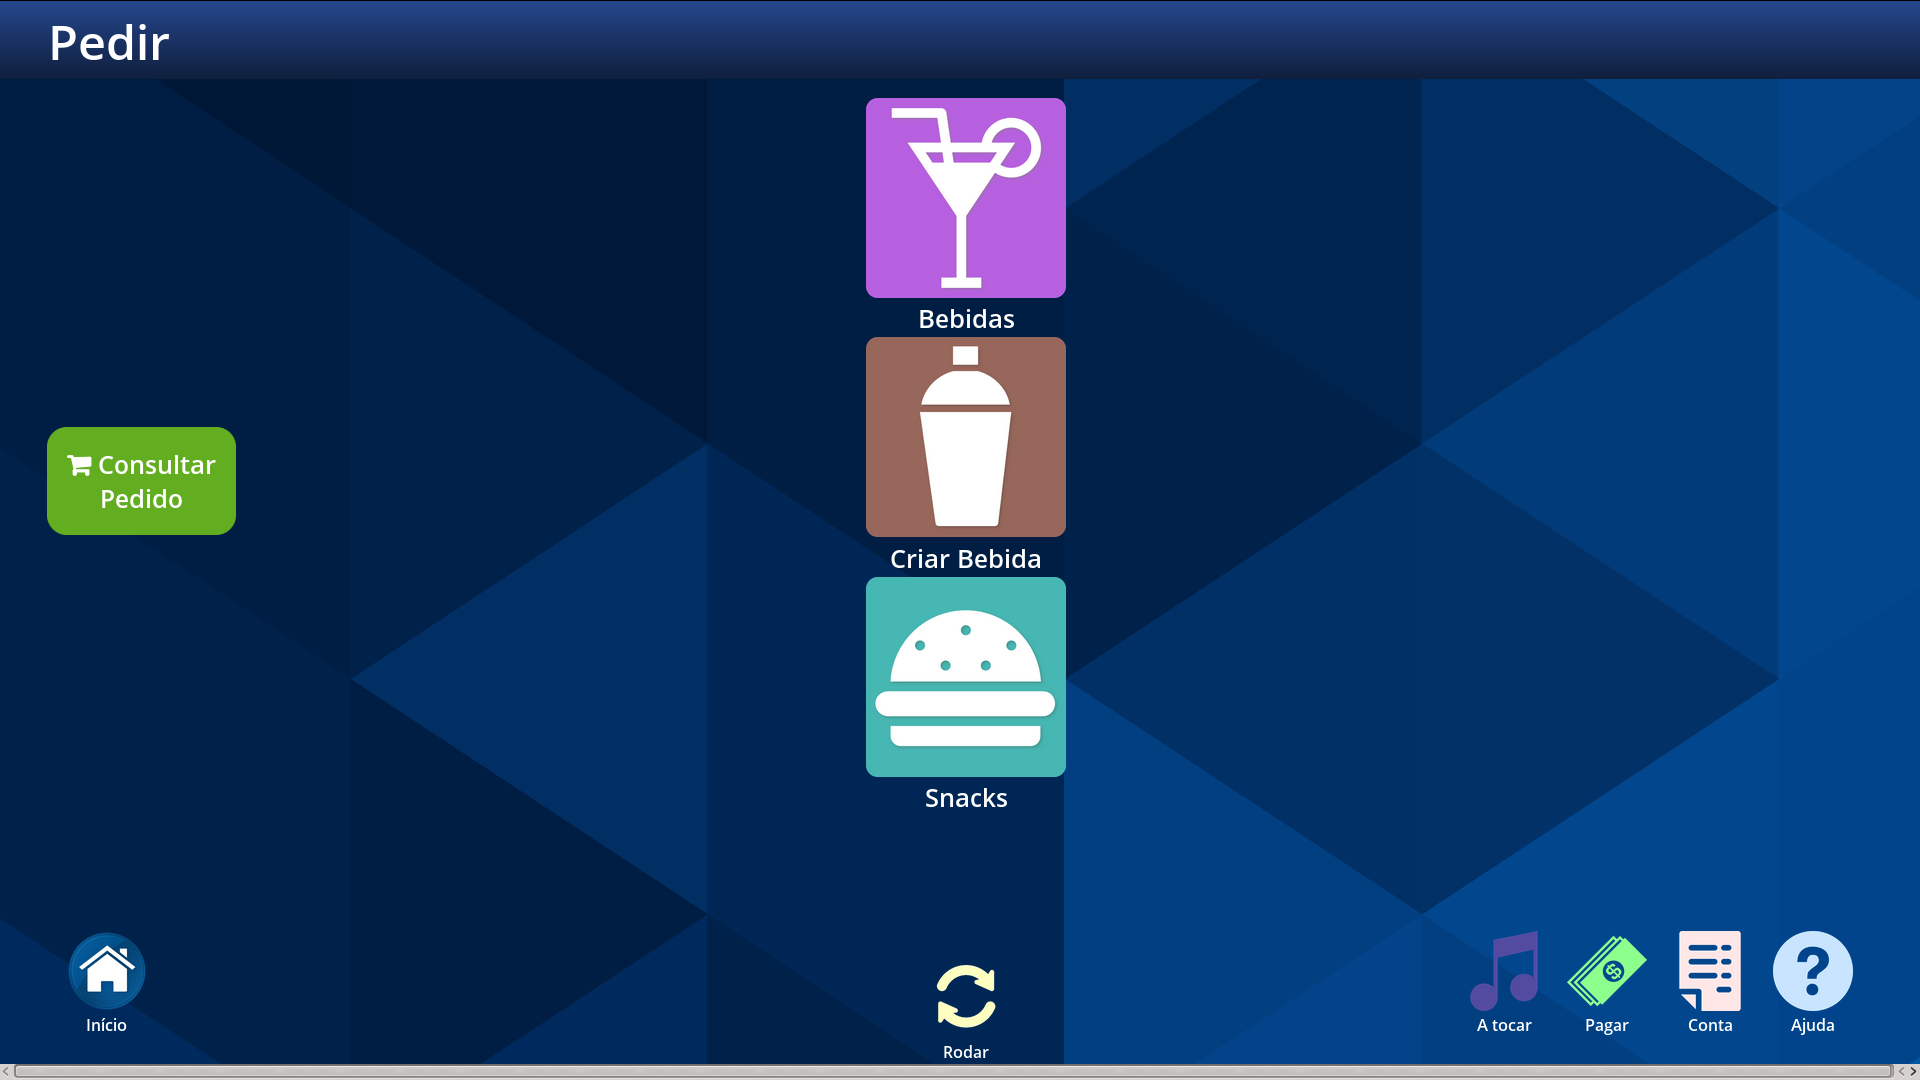
\includegraphics[width=15cm, height=8cm]{user_manual_images/order_menu.png}
\subsection{Pedir uma bebida ou snack}
Para pedir uma bebida ou um snack neste menu, o utilizador têm de pressionar o botão que lhe corresponde, sendo que aparece um menu lateral onde este pode adicionar bebidas ao carrinho.\\
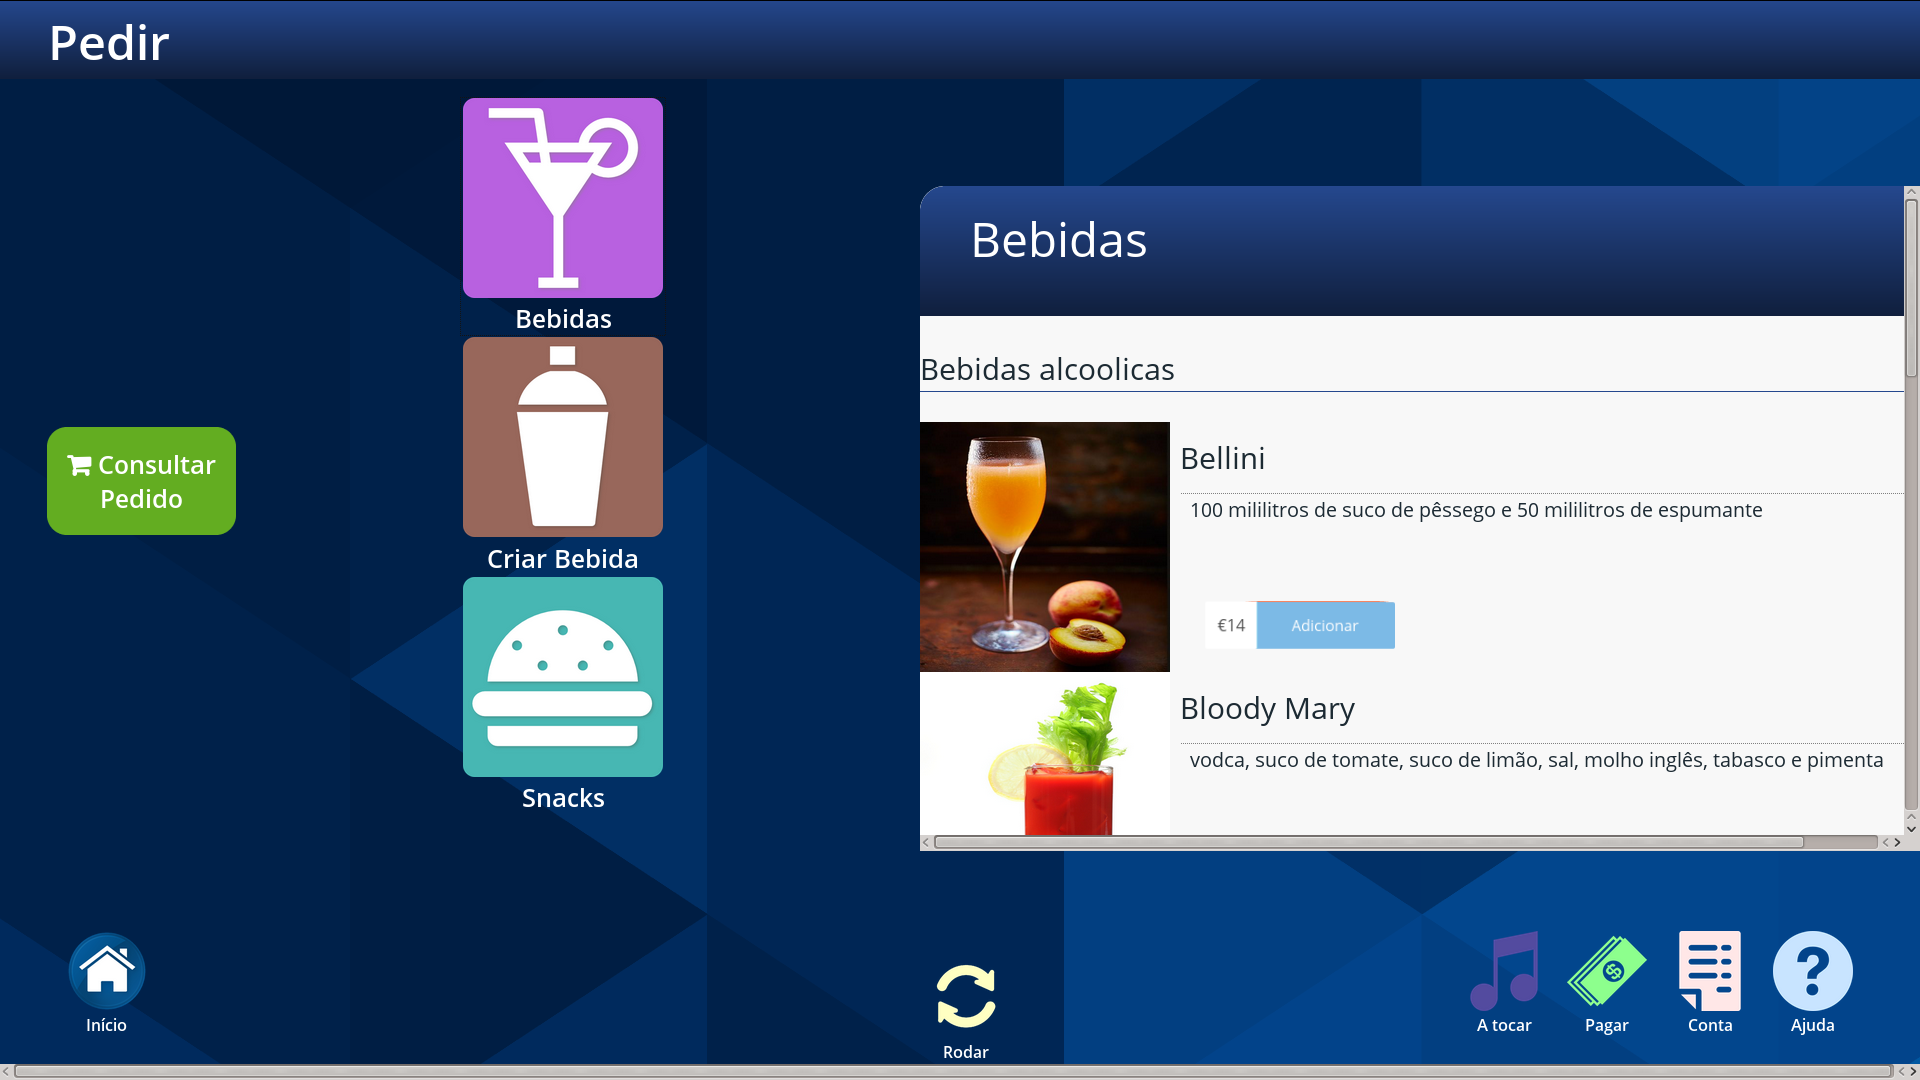
\includegraphics[width=15cm, height=8cm]{user_manual_images/drinks_submenu.png} Após ter escolhido as bebidas/snacks, para confirmar o pedido, o utilizador tem de pressionar o botão Consultar Pedido, e de seguida o botão Pedir.\\
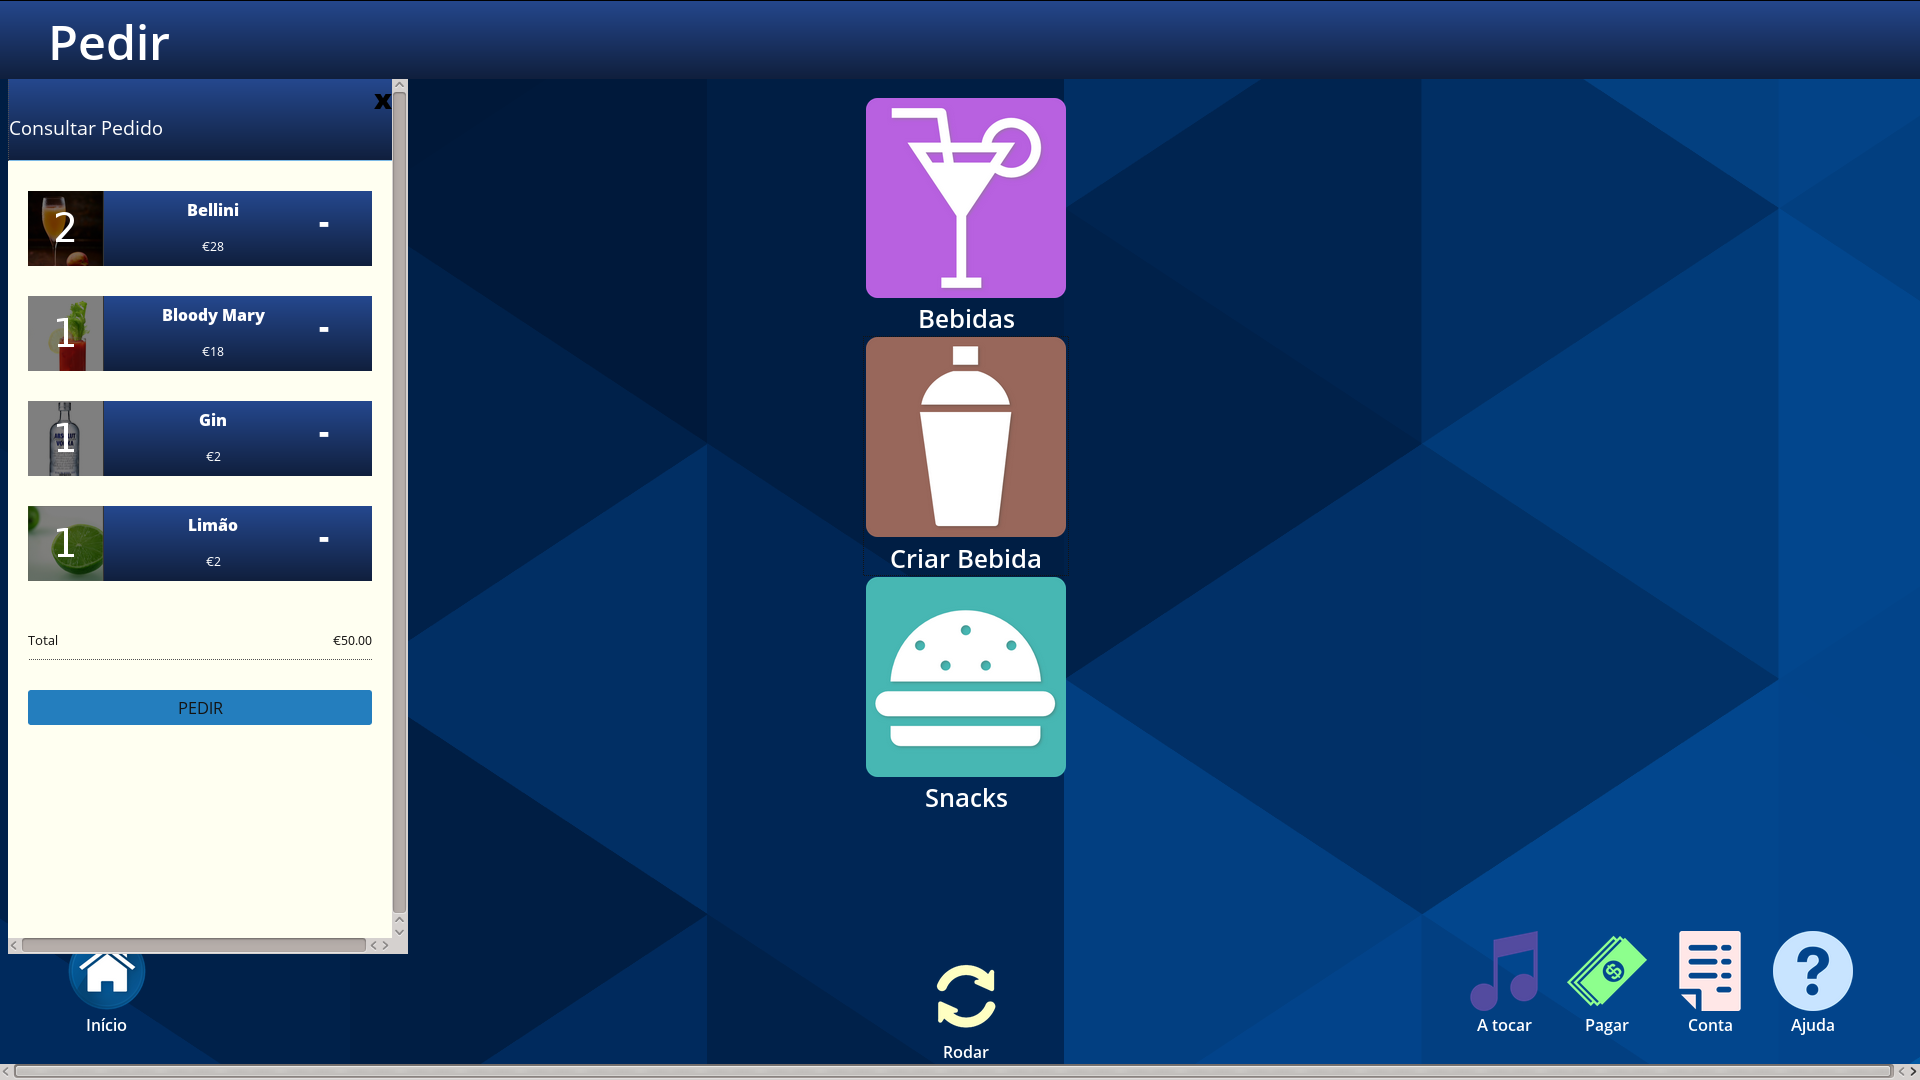
\includegraphics[width=15cm, height=8cm]{user_manual_images/ask_order_submenu.png}
\subsection{Criar uma bebida nova}
Para criar uma bebida nova, o utilizador pressiona o botão do meio do ecrã de bebidas. Tal como para pedir uma bebida ou snack já existente, aparece um ecrã lateral, em que desta vez o utilizador pode selecionar os ingredientes que vão constituir a bebida.\\
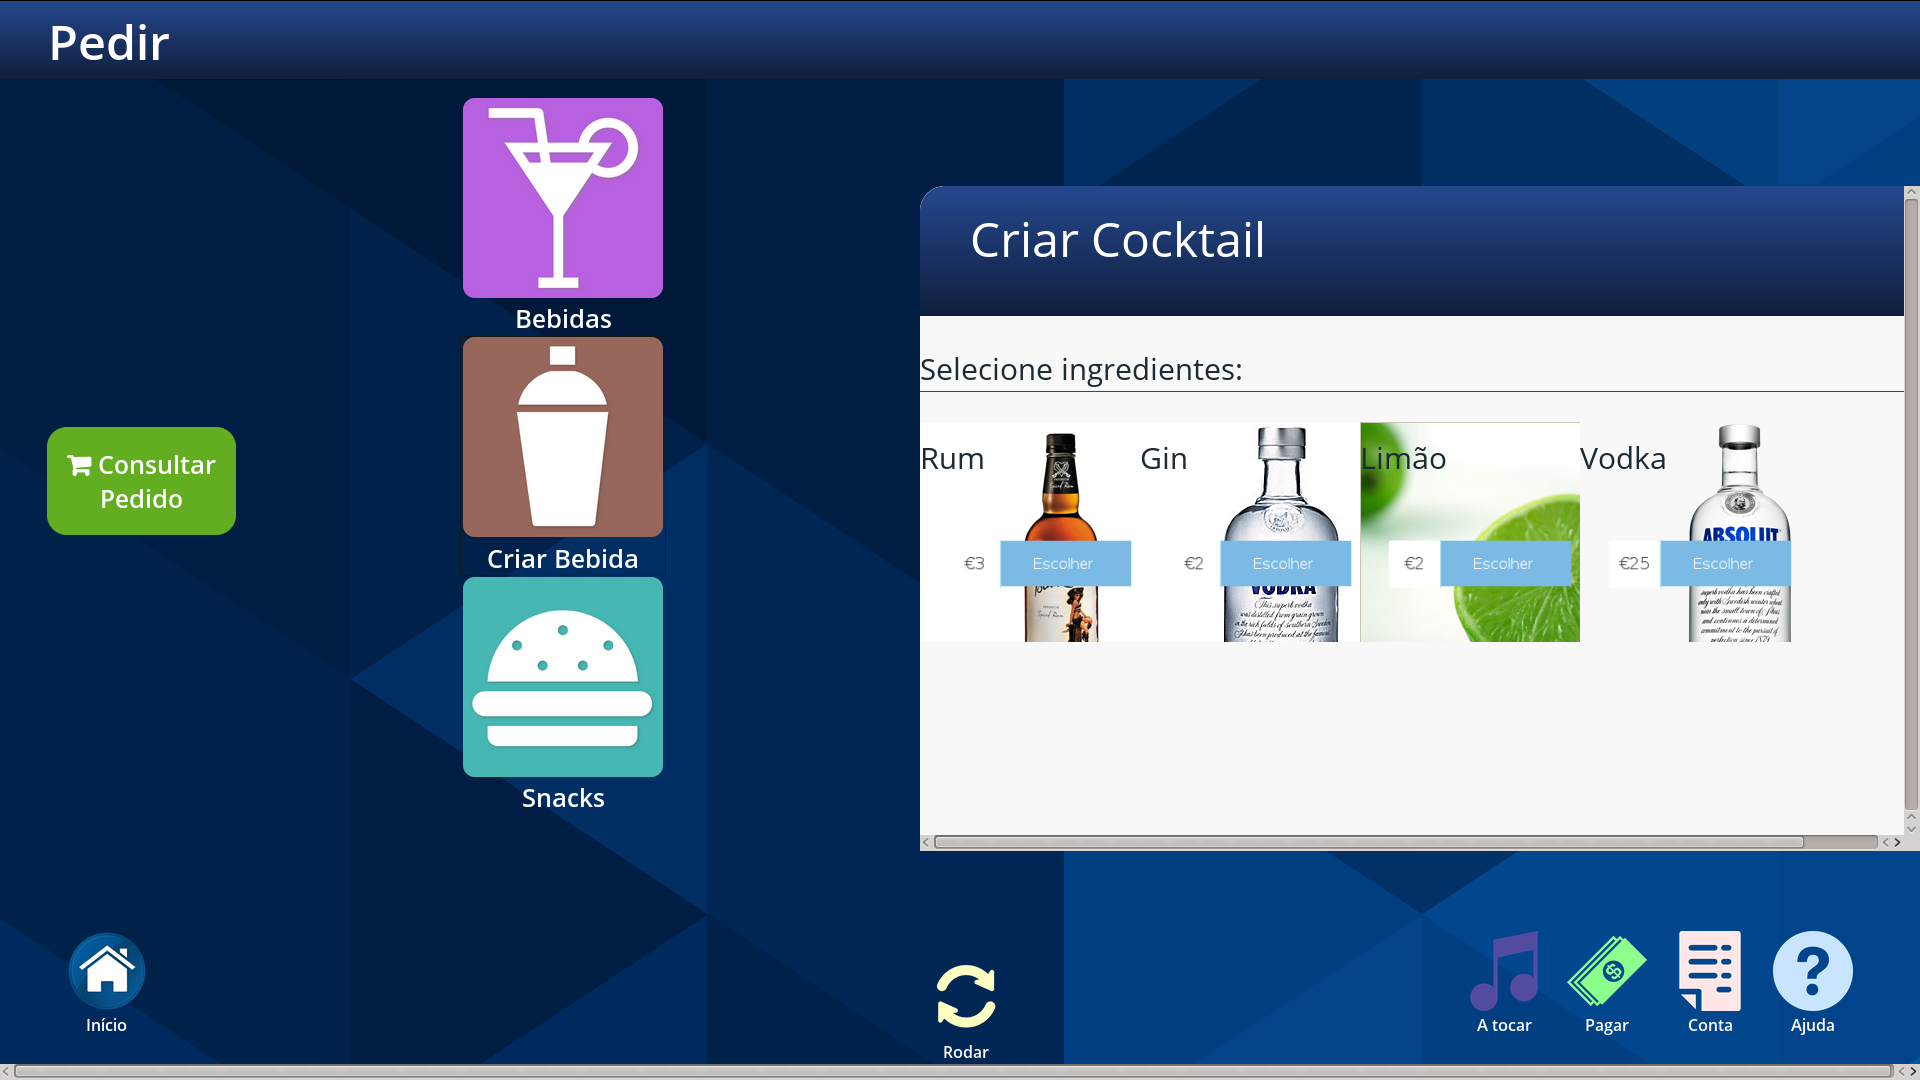
\includegraphics[width=15cm, height=8cm]{user_manual_images/create_submenu.png}.
Após um ingrediente ser seleciona, é tratado como se fosse uma bebida independente, sendo que tem de se confirmar o pedido como se fosse uma.
\subsection{Pagar}
Para pagar basta carregar no botão Pagar, sendo o utilizador direcionado  para o seguinte ecrã. \\\\ 
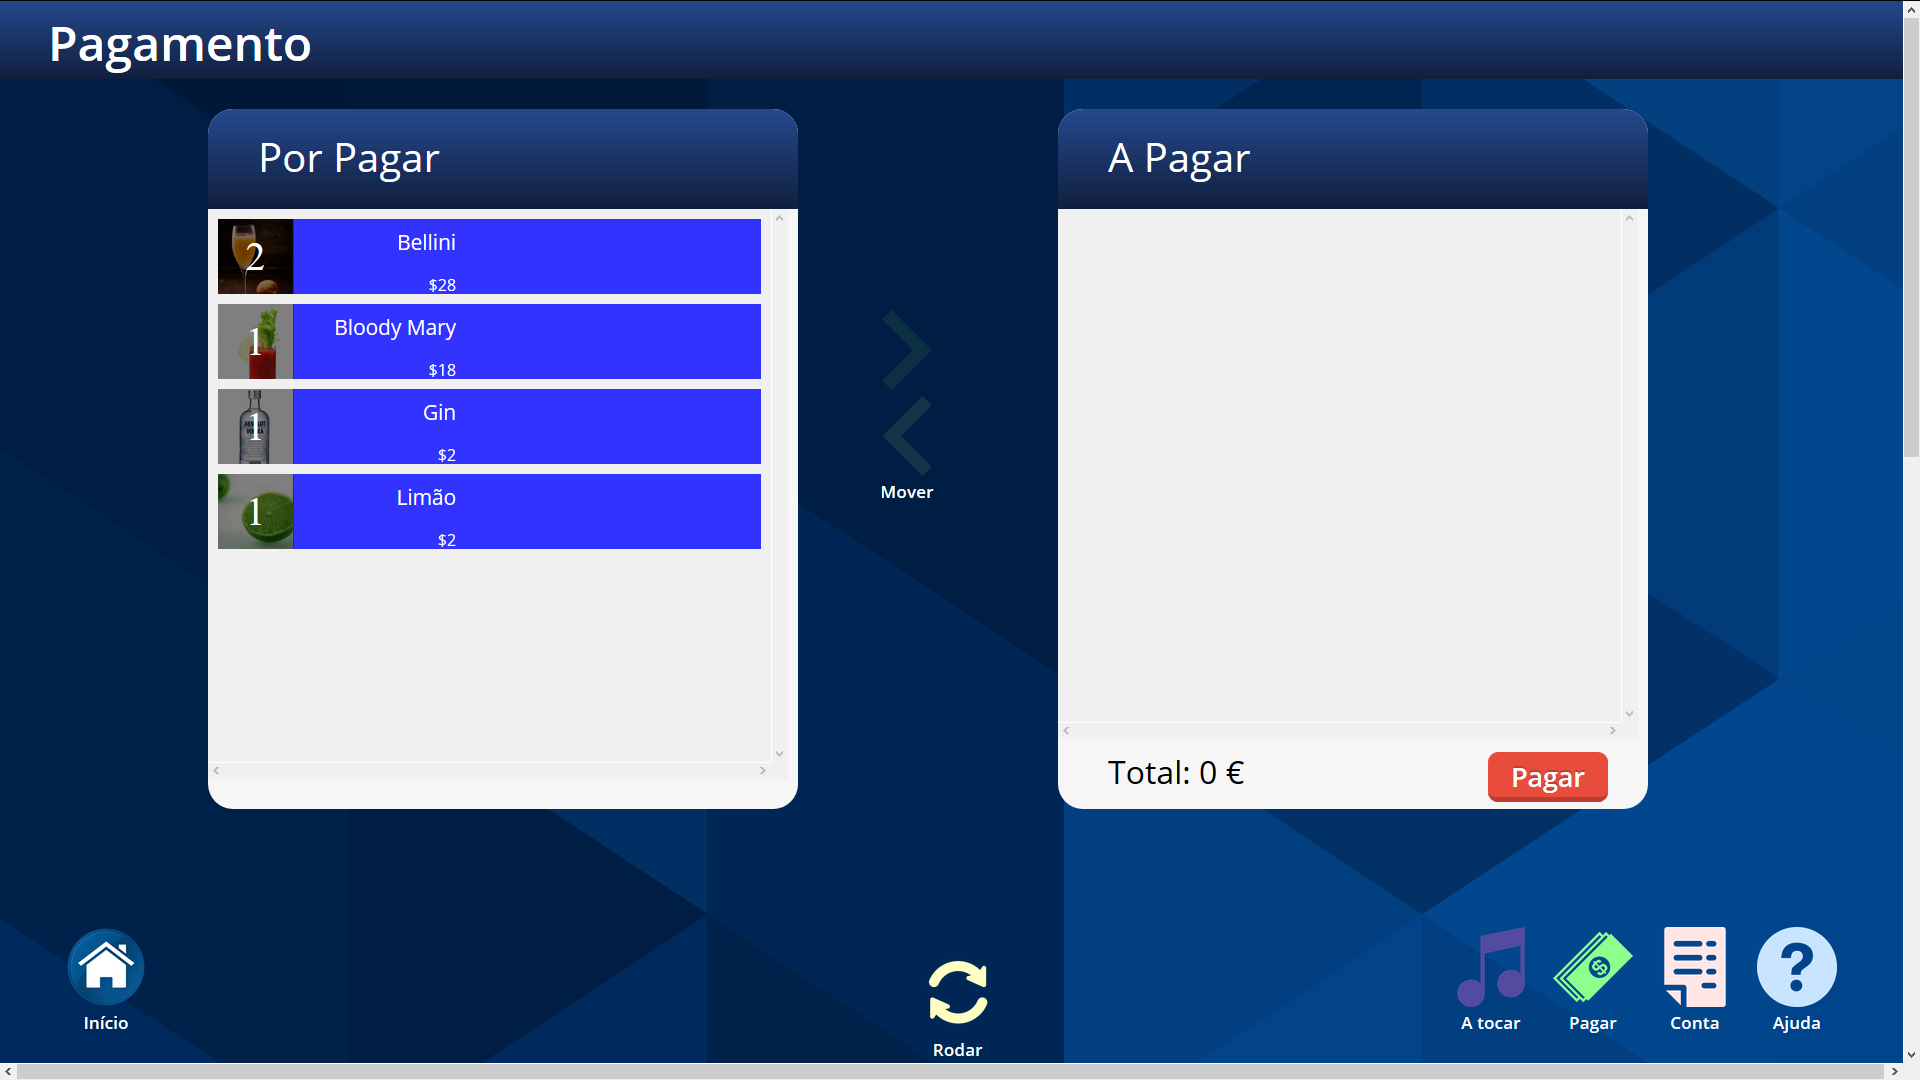
\includegraphics[width=15cm, height=8cm]{user_manual_images/pay_menu.png}
No 1º rectângulo, encontra todos os itens pedidos que ainda não foram pagos.\\
Pode escolher os itens que quer pagar, clicando neles.\\\\
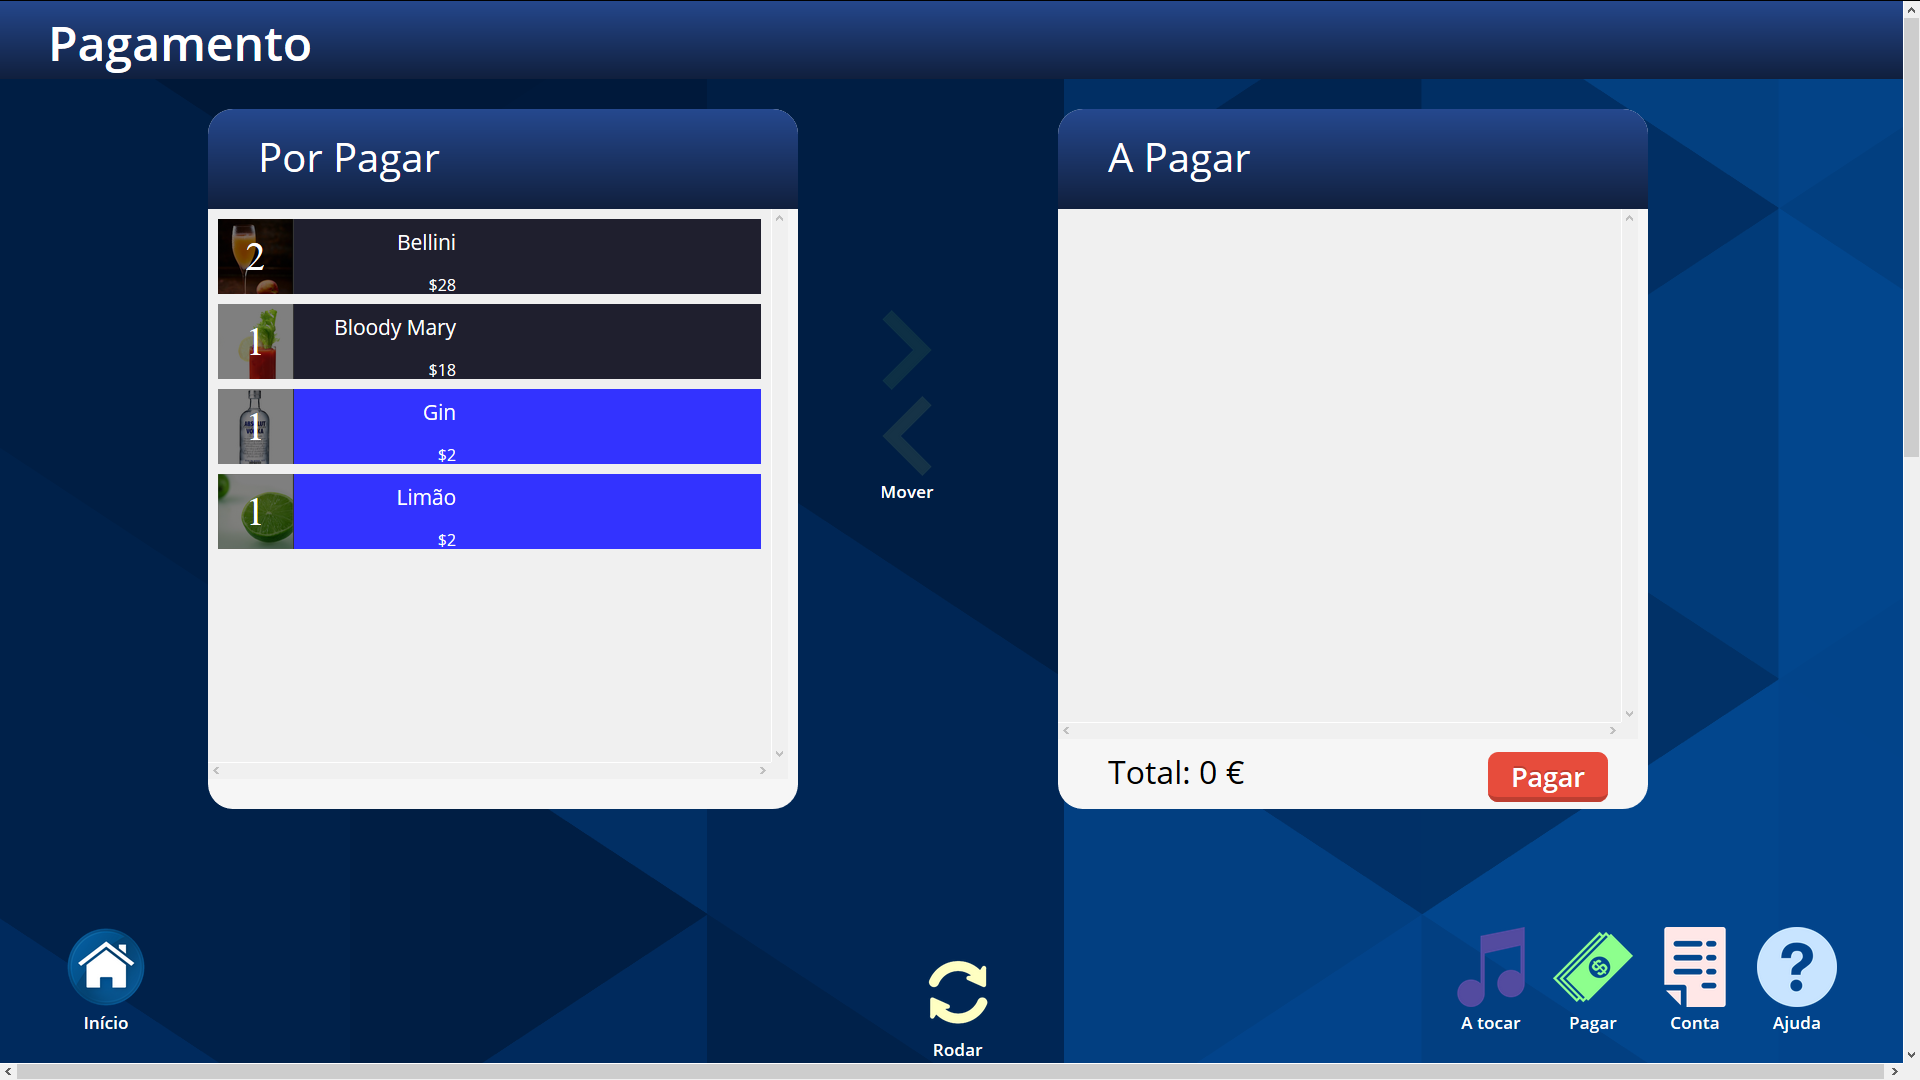
\includegraphics[width=15cm, height=8cm]{user_manual_images/select_pay.png}
Ao carregar na seta que aponta para a direita,os itens escolhidos passam para o 2ºrectângulo.\\\\
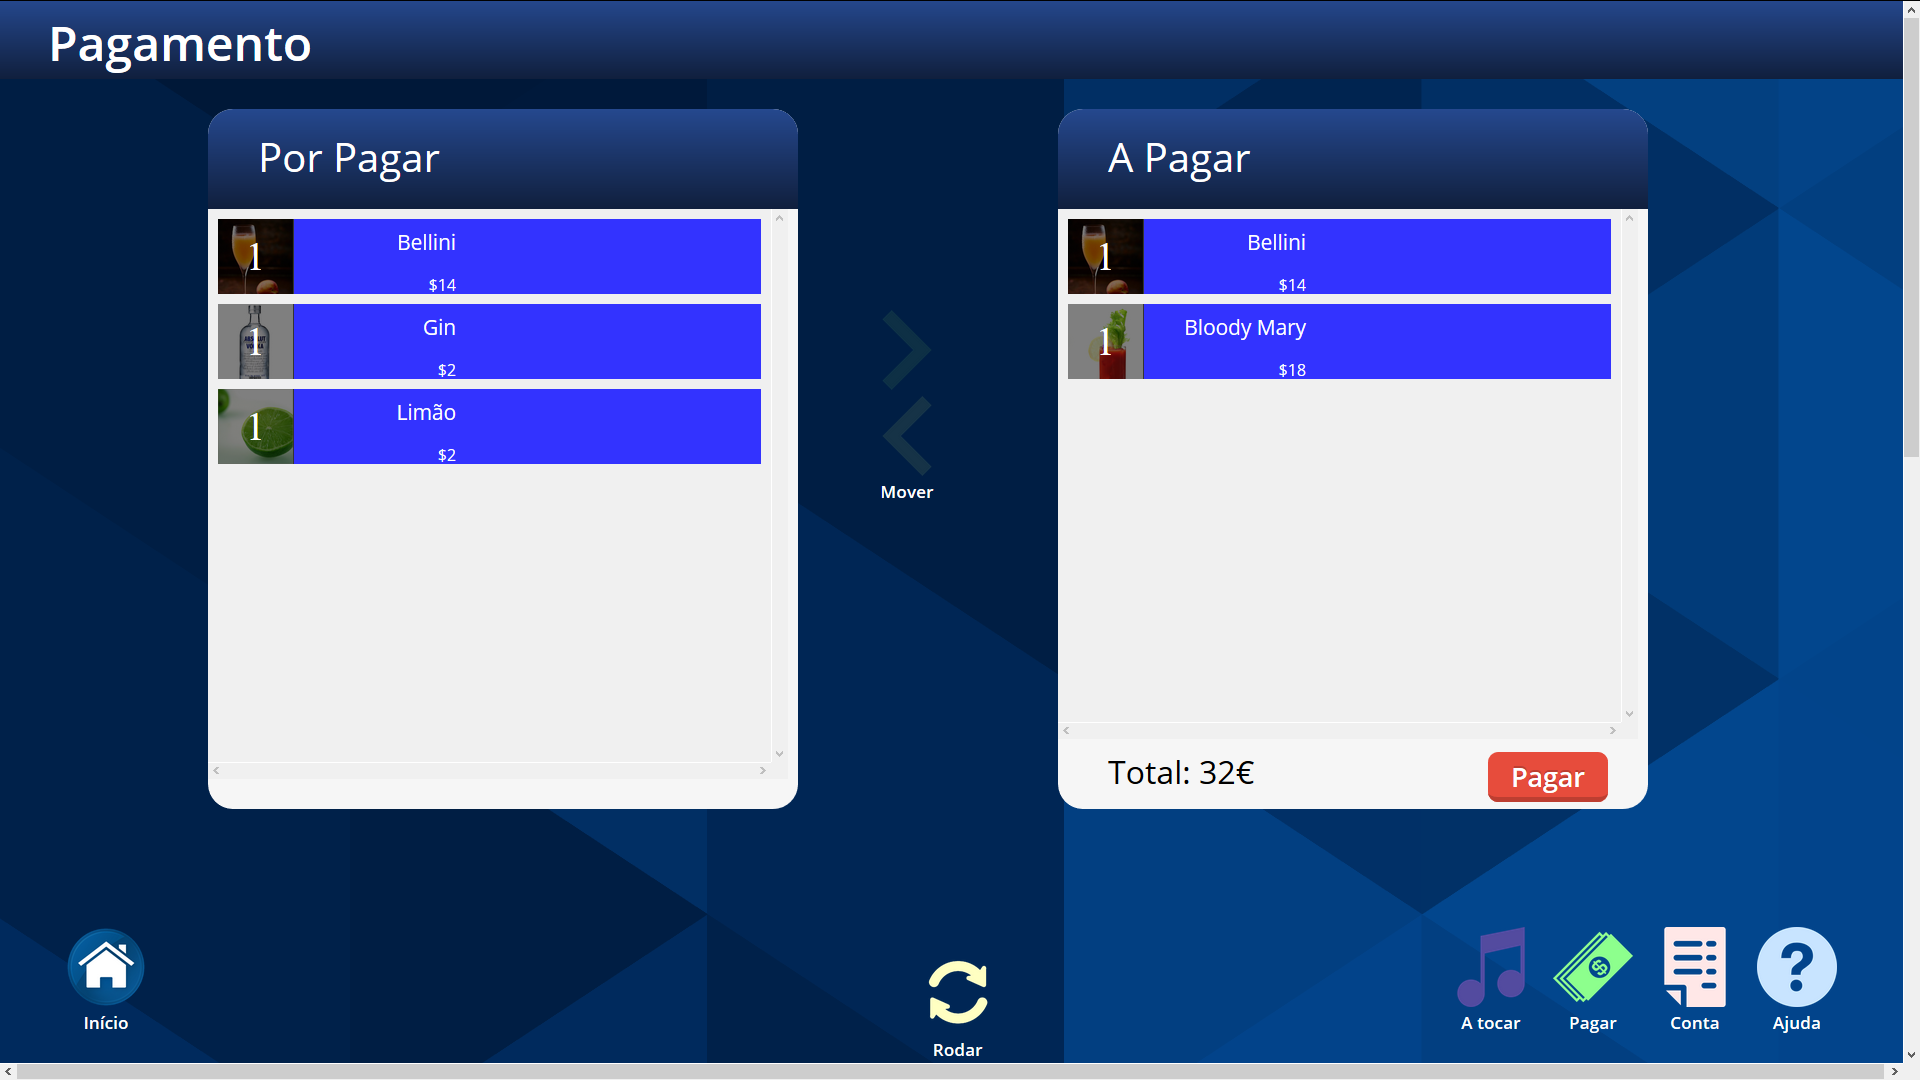
\includegraphics[width=15cm, height=8cm]{user_manual_images/moved_itens.png}
Se houverem itens que afinal não pretende pagar, clique em cada um e depois carregue na seta a apontar para a esquerda. Isto passa esses itens para o 1º rectângulo.\\
Ao clicar no botão pagar no 2ºrectângulo, é-lhe mostrado os diferentes tipos de pagamento efetuando assim o pagamento dos itens selecionados anteriormente.\\\\
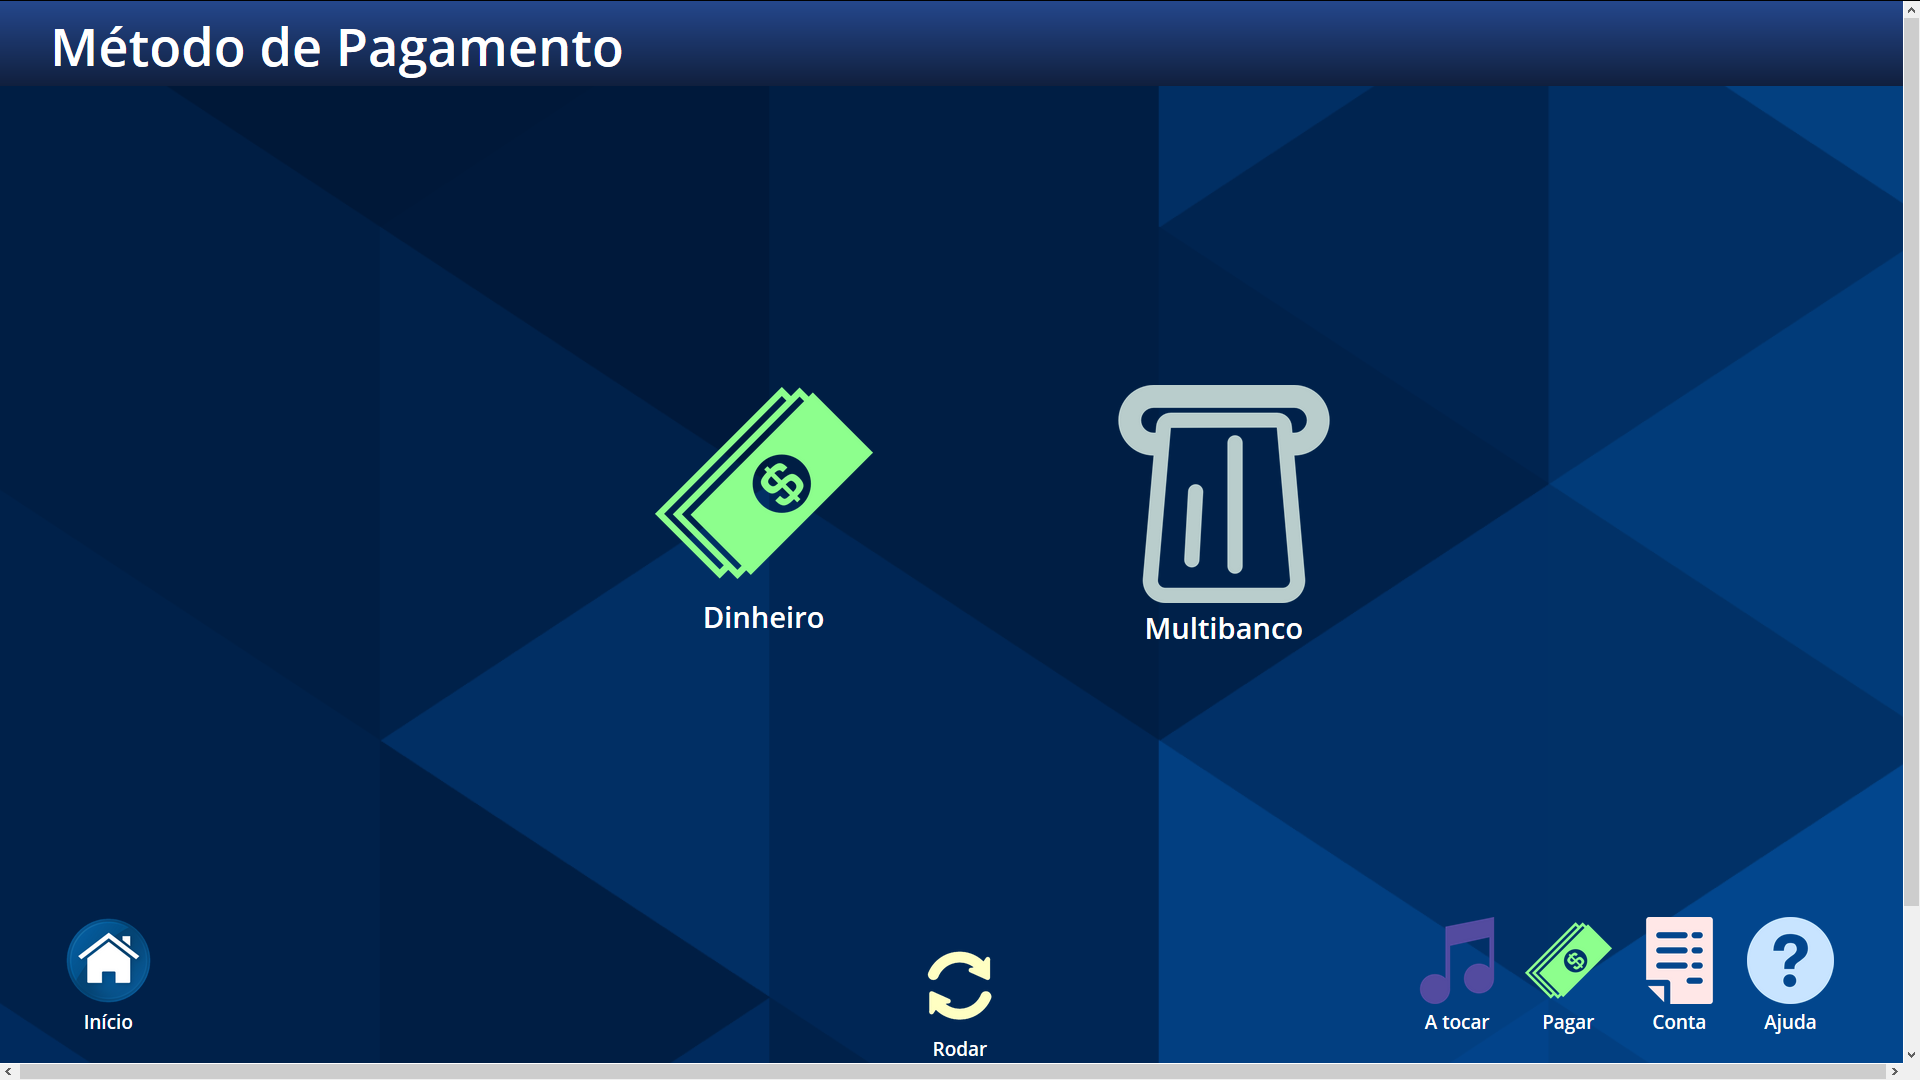
\includegraphics[width=15cm, height=8cm]{user_manual_images/payment_methods.png}
\subsection{Pedir uma bebida em qualquer ecrã}
Para facilitar a vida ao utilizador, é também possivel pedir mais uma bebida de uma das bebidas que já estejam na conta. Para tal o utilizador só tem de pressionar o botão para visualizar a conta, presente em todos os ecras no parte inferior do ecrã, e pressionar o botão + (mais) ao lado da bebida que pretende.\\
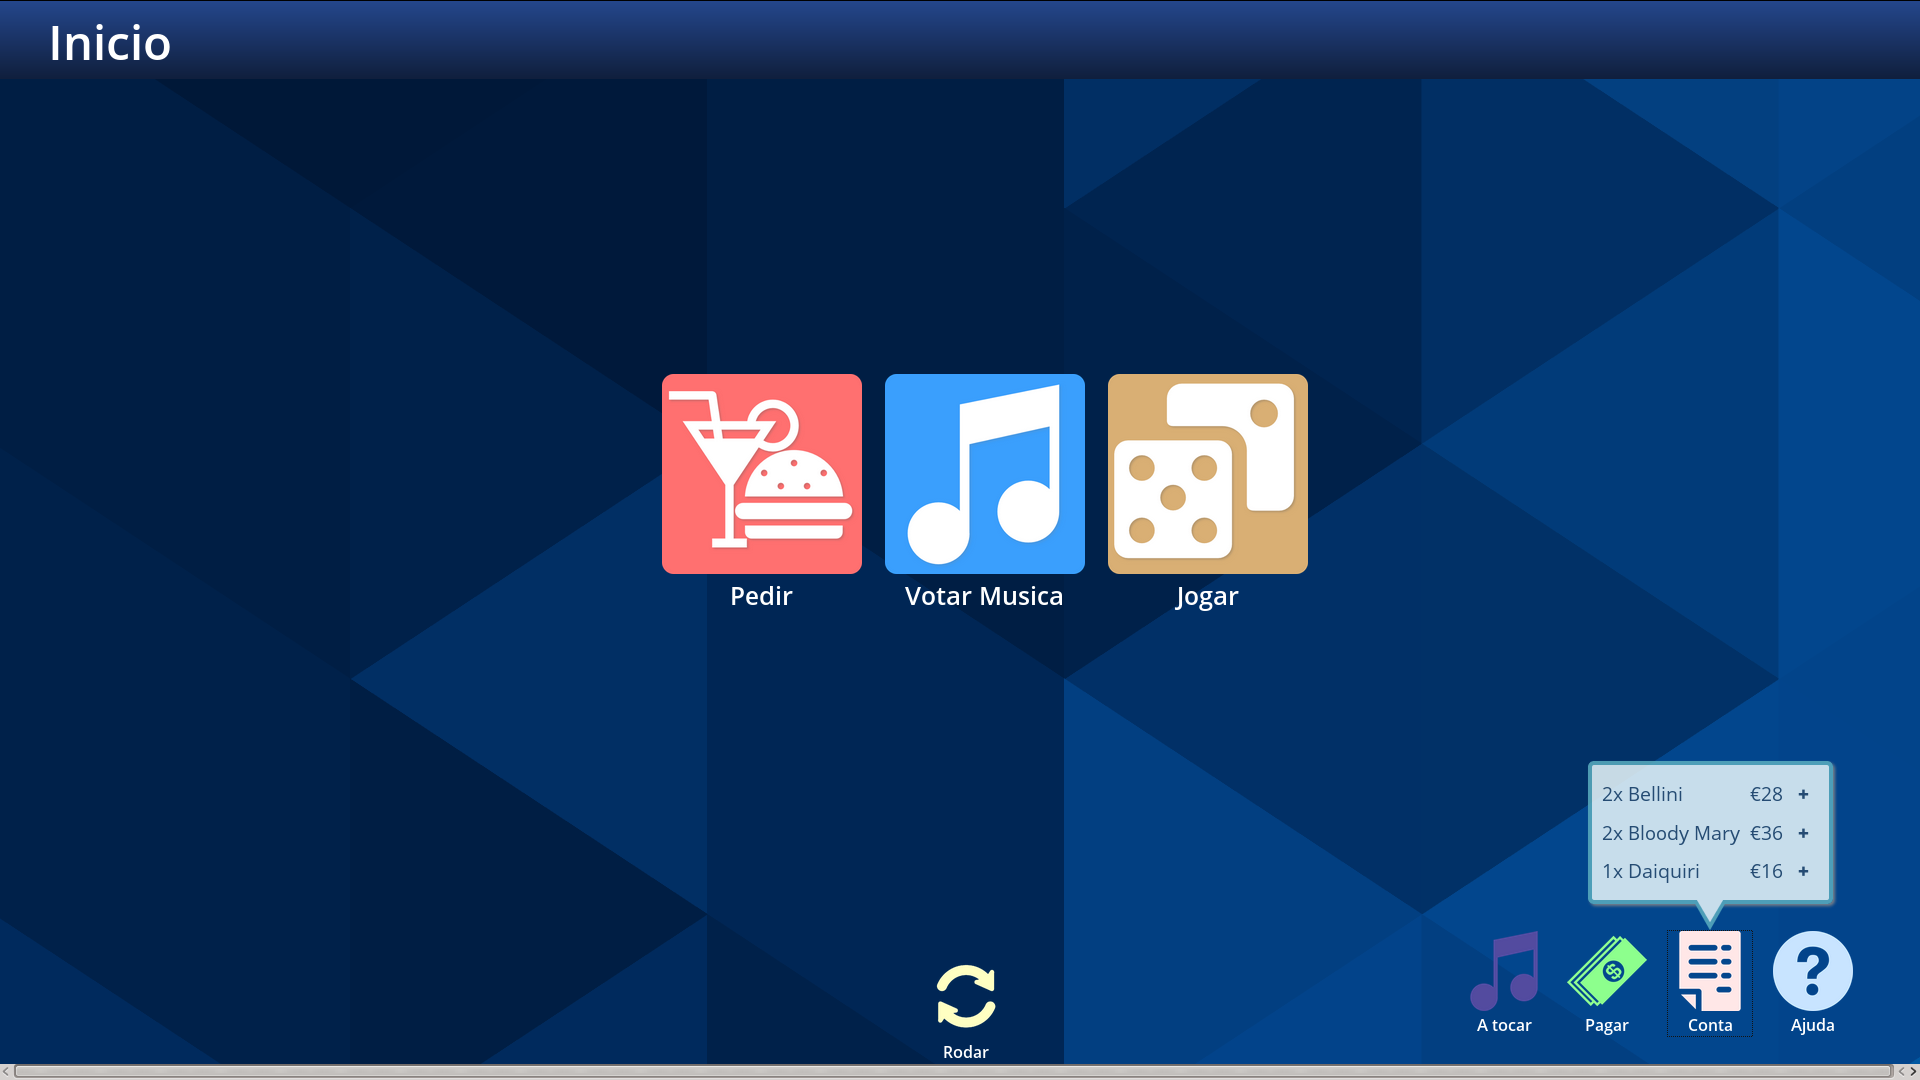
\includegraphics[width=15cm, height=8cm]{user_manual_images/order_ballon.png}.
\section{Música}
\subsection{Escolher e votar numa música}
Para navegar pelo menu coverflow, o utilizador manter o dedo pressionado em cima de qualquer um dos albums e arrastá-lo para um dos lados para andar com os albuns para o lado. Assim que o ecra tiver centrado no album desejado, basta votar no botão Votar. Aparecera um popup a confirmar o voto.\\\\
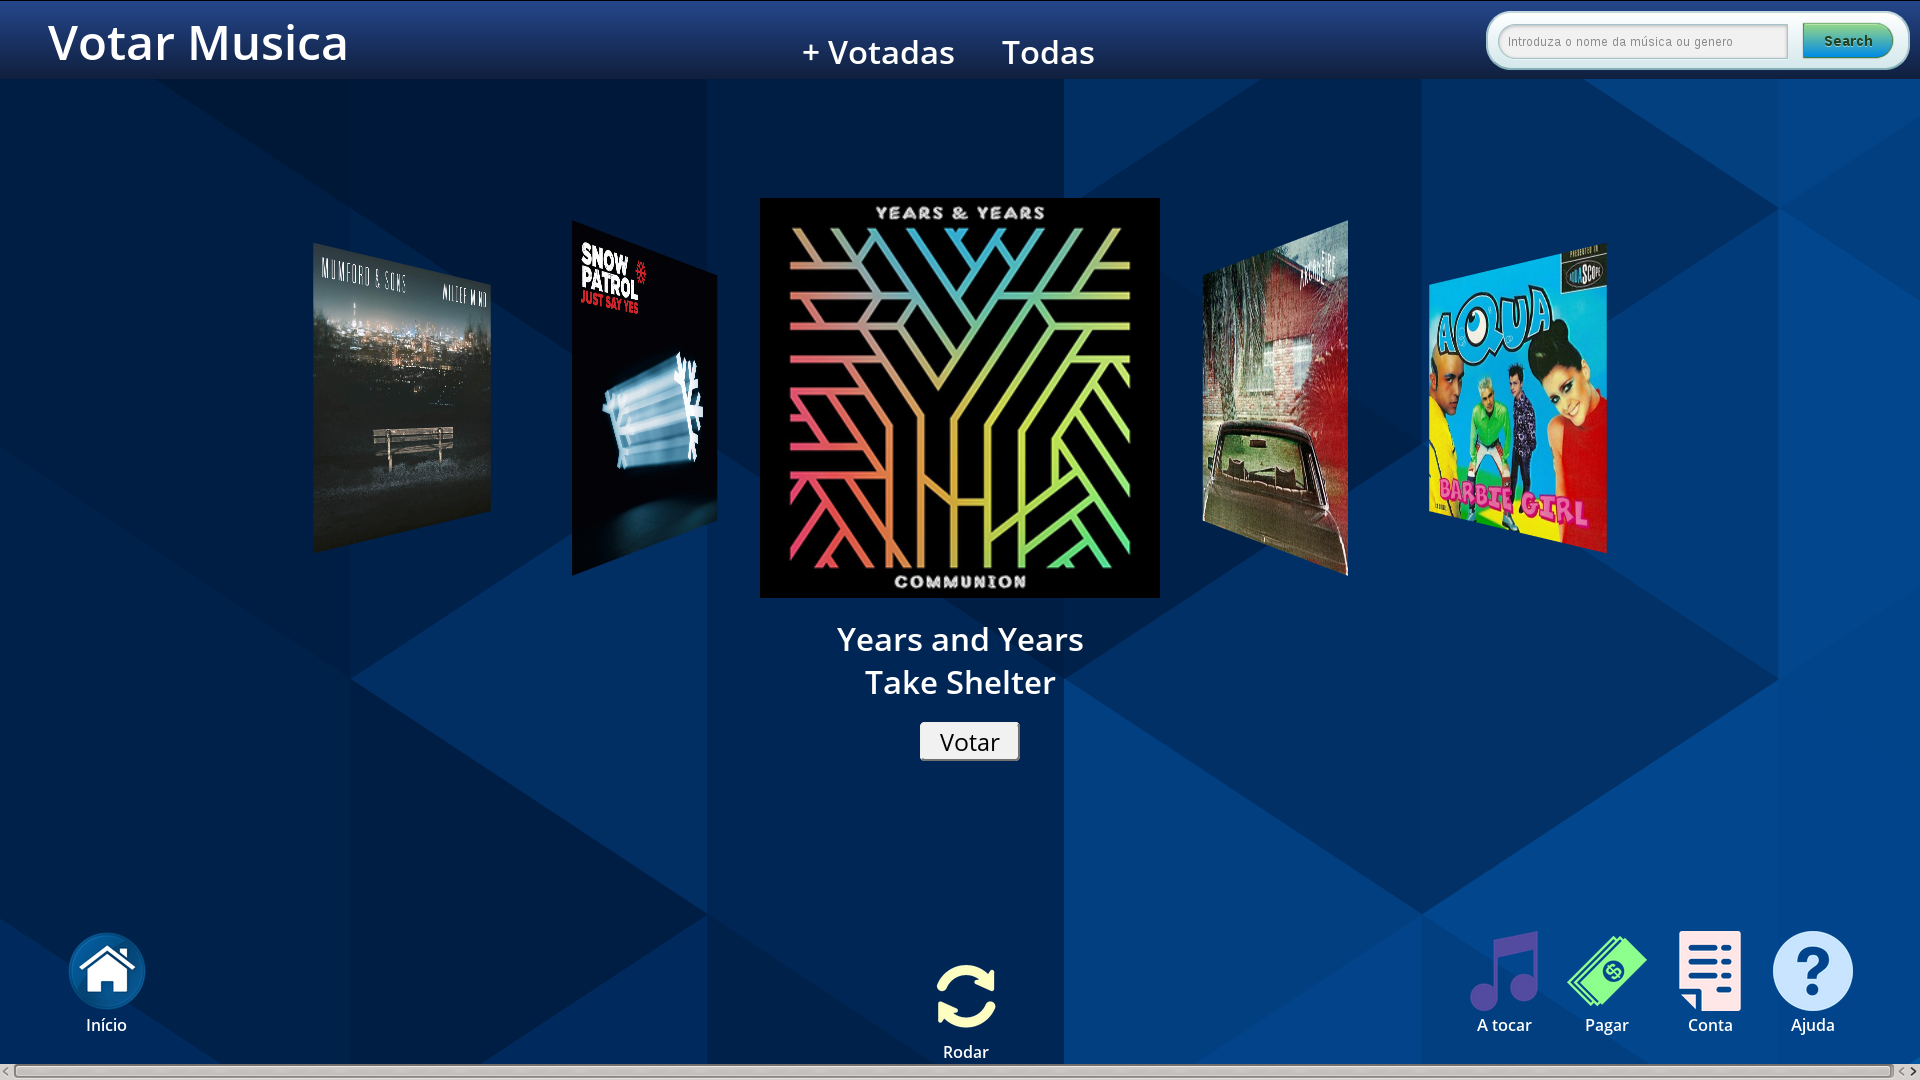
\includegraphics[width=15cm, height=8cm]{user_manual_images/vote_menu.png}.
\subsection{Ordenar por popularidade}
Para ver as músicas mais votadas no momento, basta pressionar no botão + Votadas. As músicas no menu coverflow mudaram e aparecem ordenadas por numero de votos, com as respetivas percentagens de votos em cima. Para votar, tal como para o caso geral, basta pressionar no botão Votar.\\
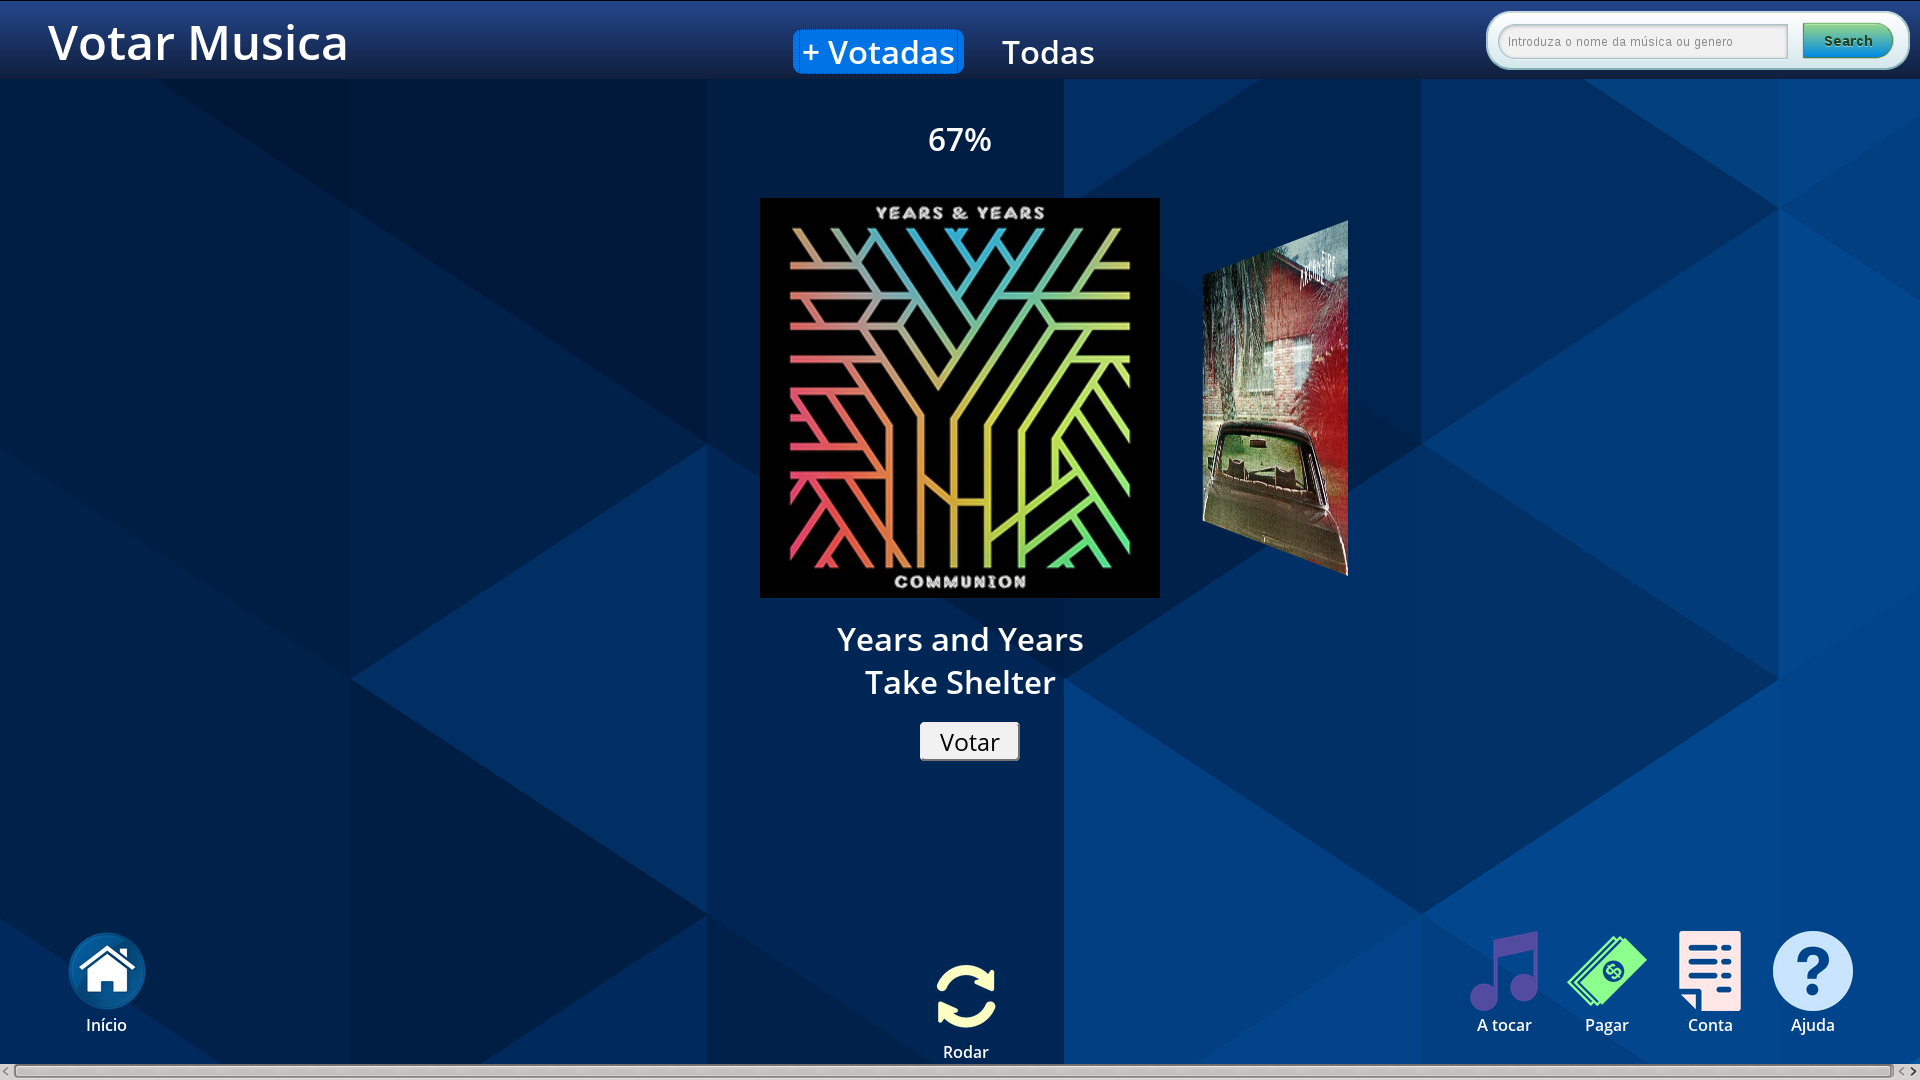
\includegraphics[width=15cm, height=8cm]{user_manual_images/most_voted.png}.
\subsection{Procurar músicas}

\subsection{Ver atual e próxima música}

\section{Jogos}
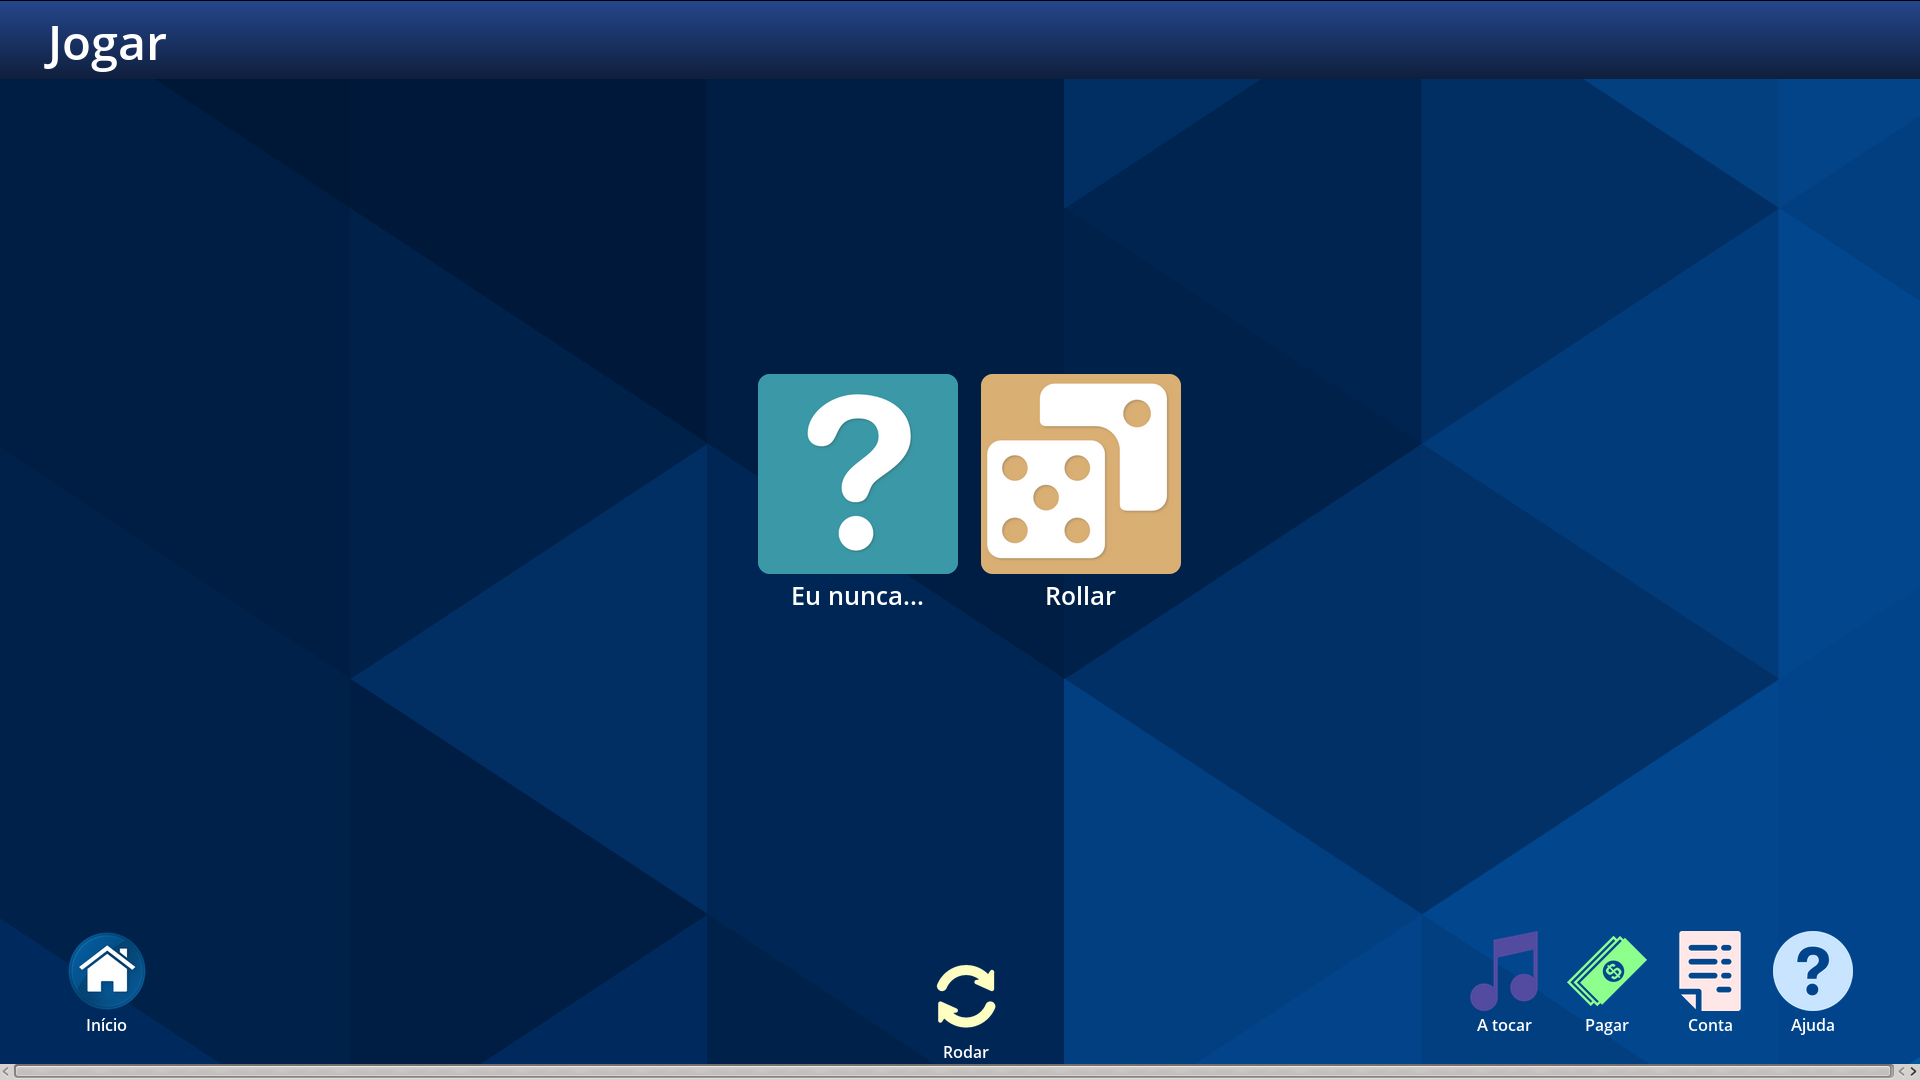
\includegraphics[width=15cm, height=8cm]{user_manual_images/games_menu.png}
Nos Jogos são apresentados 2 jogos, o Eu nunca... e o Rollar.
Em cada jogo existe o botão de Ajuda que explica as regras do jogo (canto inferior direito), e um botão para escolher uma mesa com quem jogar (explicação na secção Convidar outra mesa), um botão Início (canto inferior esquerdo) que conduz o utilizador ao ecrã principal e uma seta para voltar ao ecrã anterior (canto superior esquerdo).
\subsection{Escolher um jogo}
Para escolher um jogo basta no menu inicial clicar no botão Jogar, o que leva o utilizador ao menu Jogar apresentado na figura anterior.
O utilizador pode, de seguida, escolher um dos jogos disponibilizados.
\subsection{Eu nunca...}
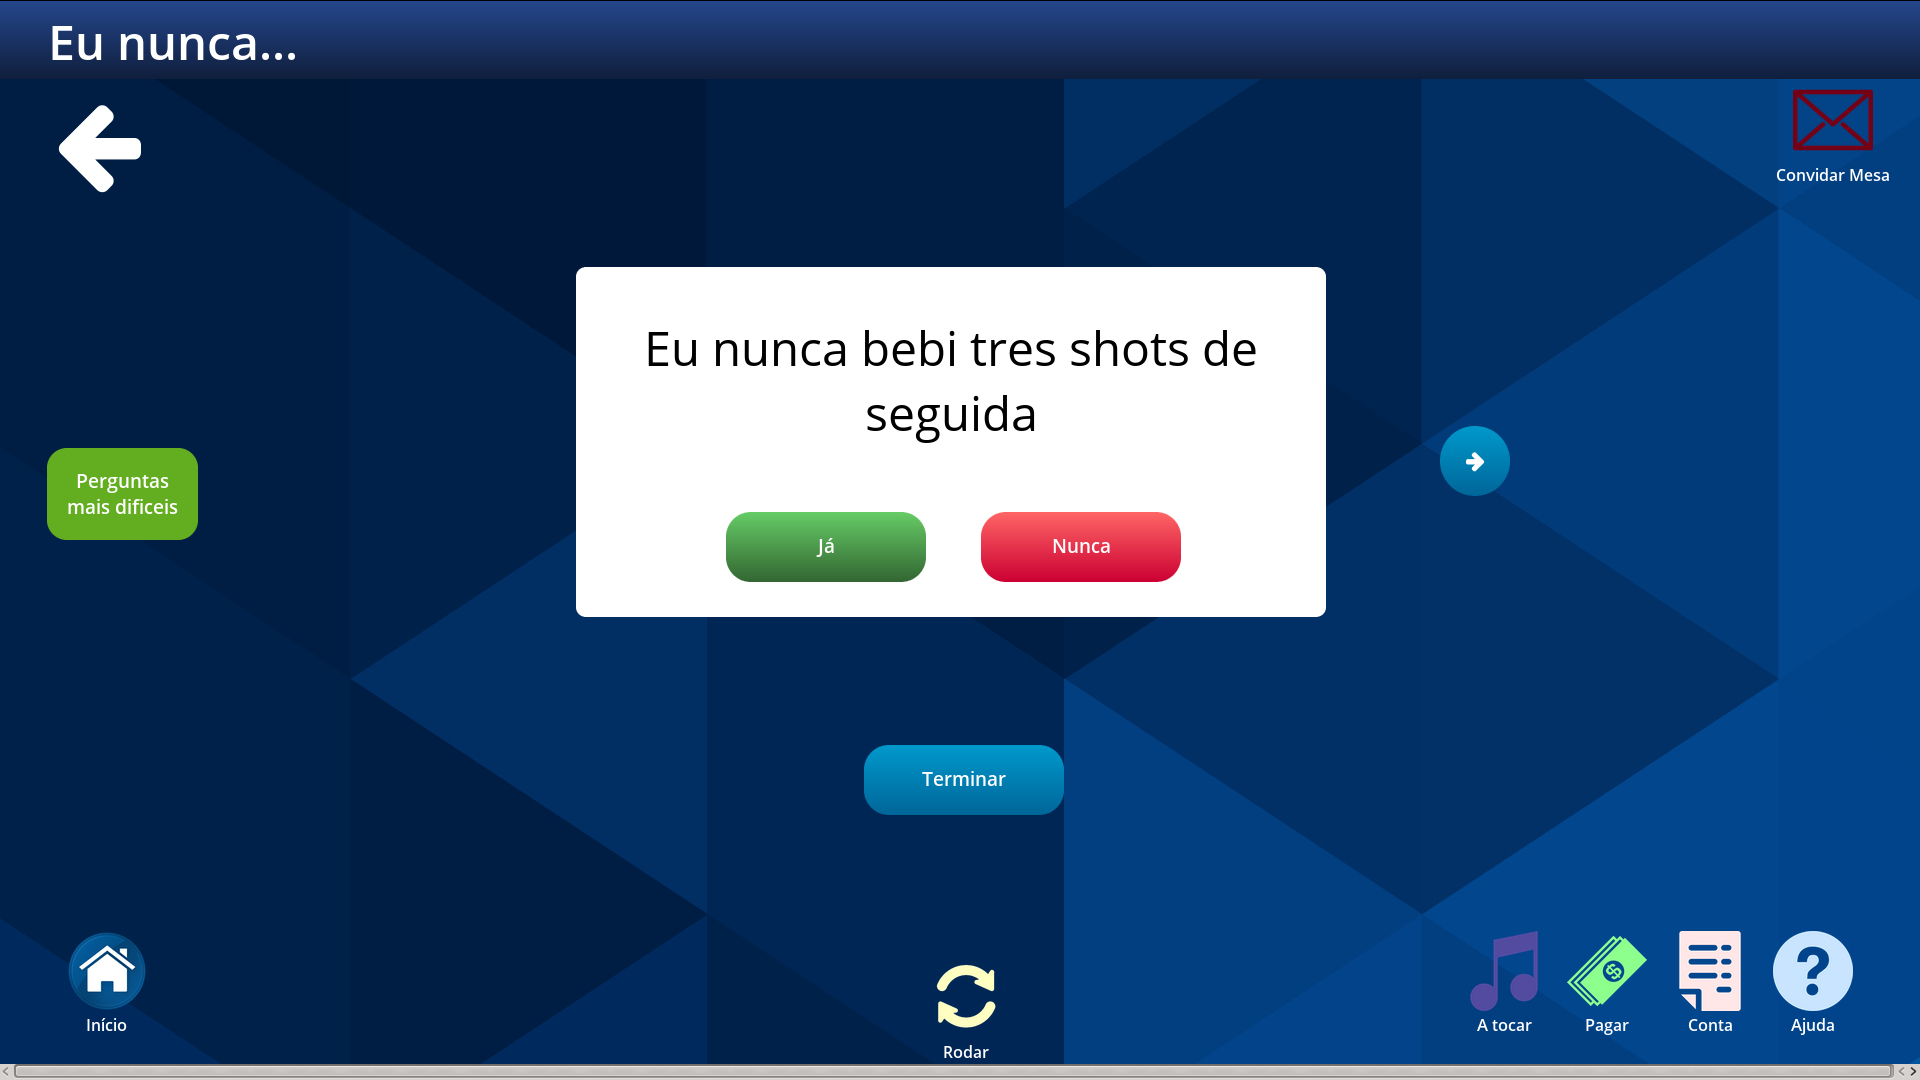
\includegraphics[width=15cm, height=8cm]{user_manual_images/i_never_game.png}
Neste ecrã, tudo o que se encontra no rectângulo central faz parte do jogo; existe um botão Início, uma seta (explicação de cada na secção Jogos)e o botão para convidar uma mesa (explicação na secção Convidar outra mesa).
O botão Perguntas mais difíceis, ao ser clicado, apresenta uma lista das perguntas com mais "Nuncas" respondidos.\\\\
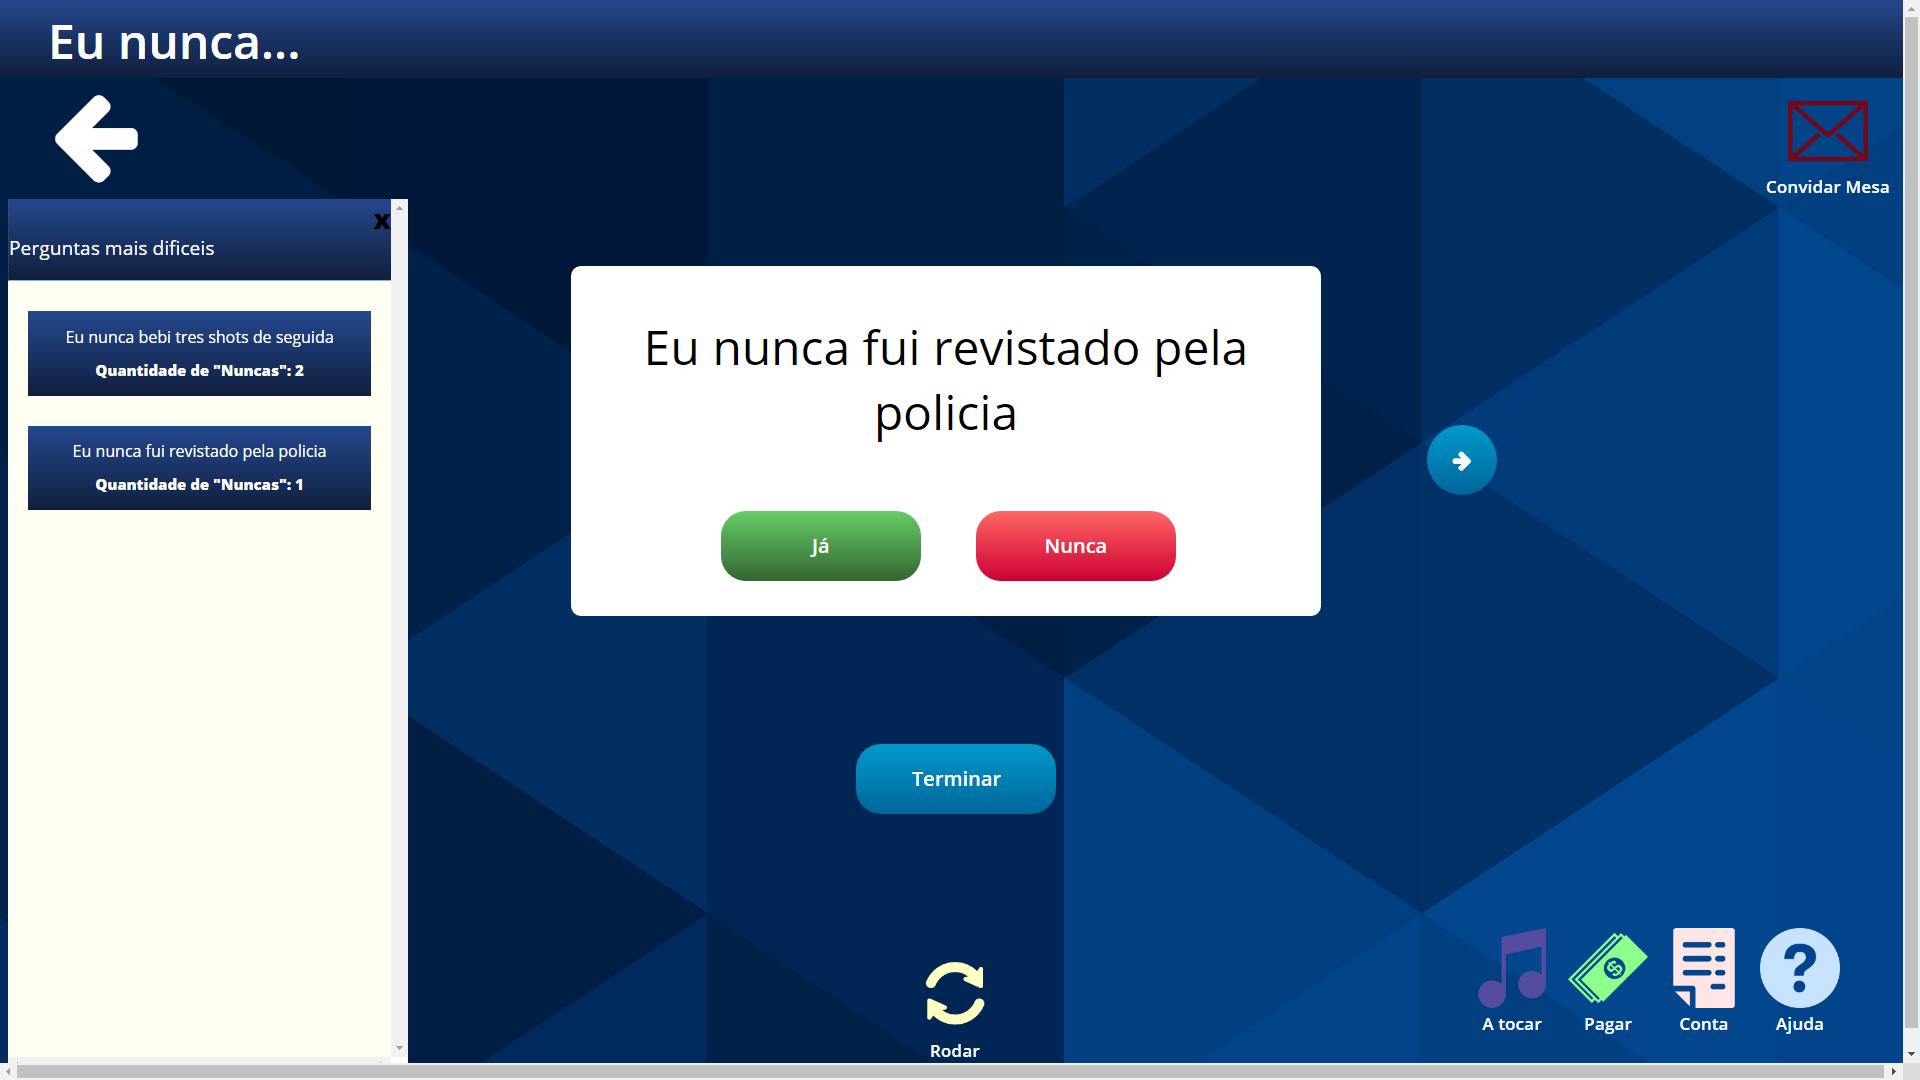
\includegraphics[width=15cm, height=8cm]{user_manual_images/hard_questions.png}
\subsection{Rolar}
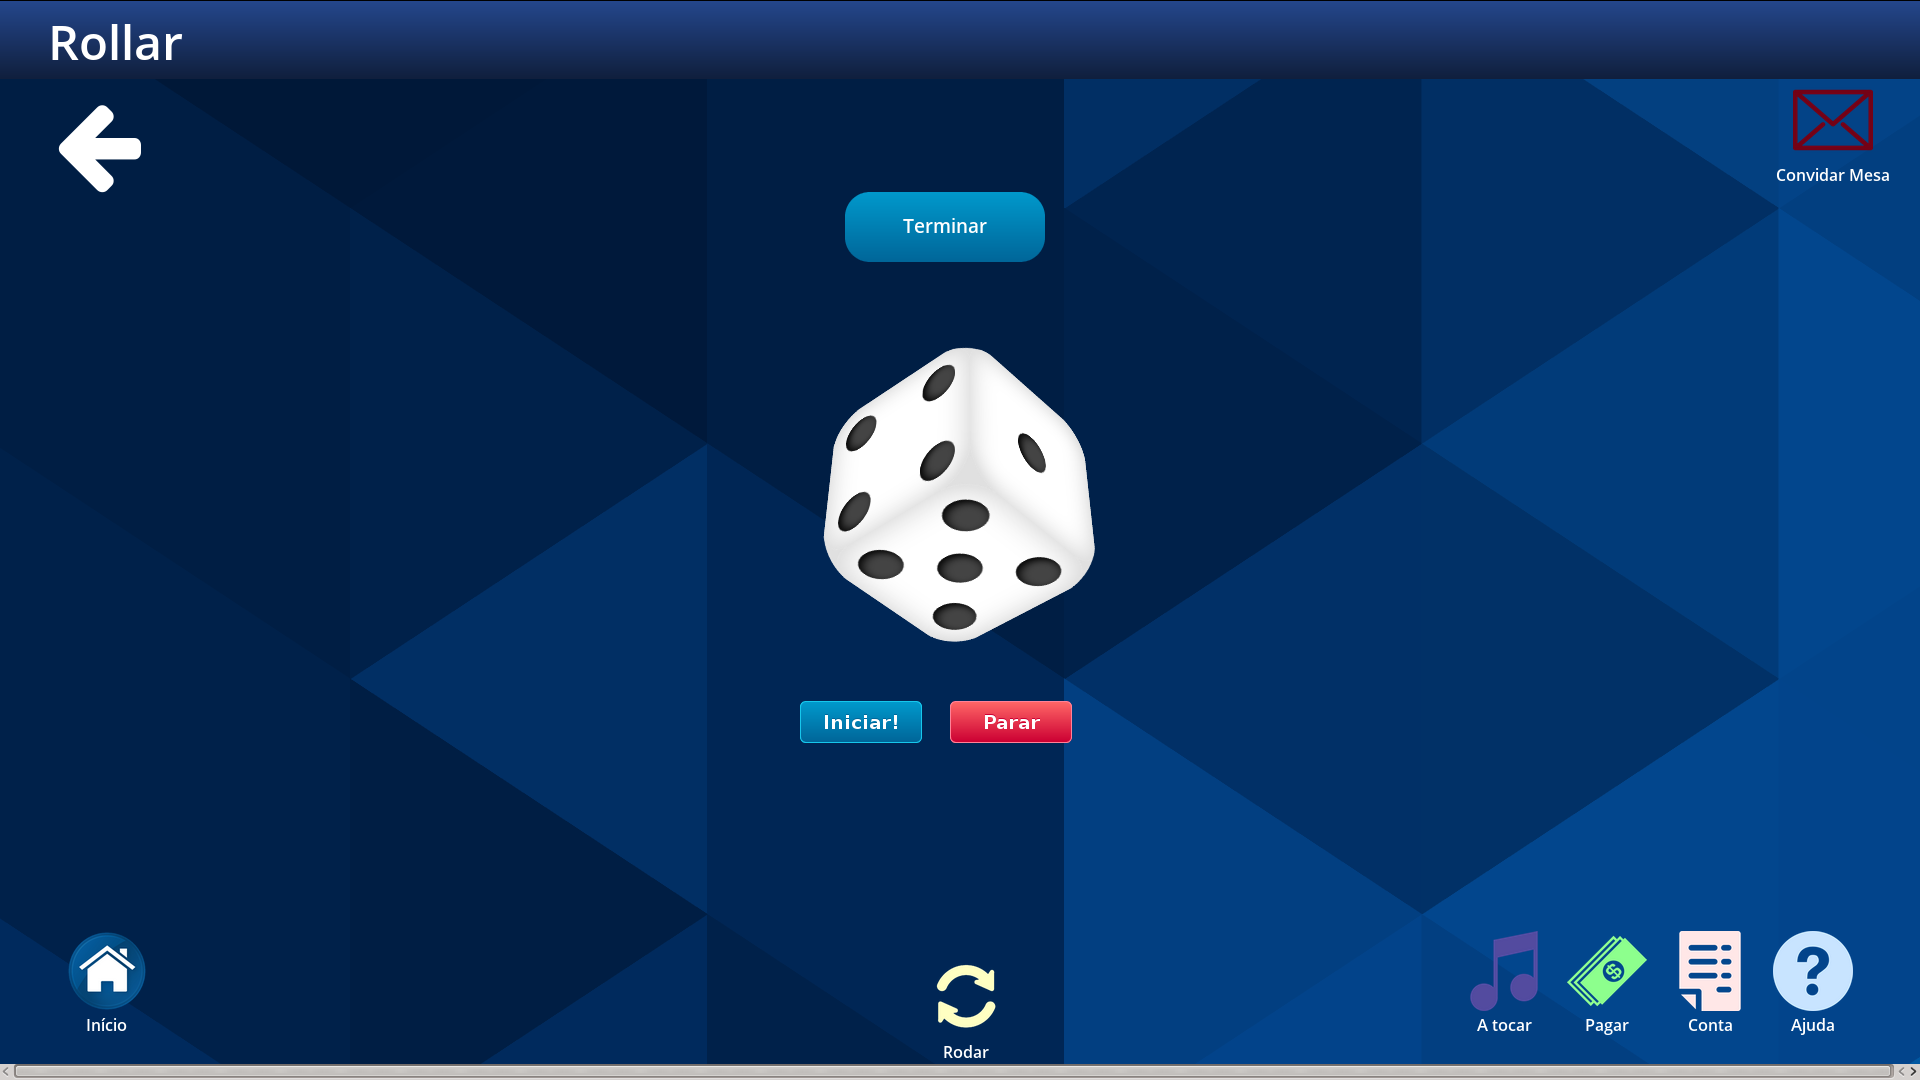
\includegraphics[width=15cm, height=8cm]{user_manual_images/roll_game.png}
Neste ecrã, os botões Iniciar! e Parar fazem parte do jogo; existe um botão Início (canto inferior esquerdo) uma seta, o botão para convidar uma mesa e o botão Ajuda (explicação de cada na secção jogos).
\subsection{Convidar outra mesa}
Para convidar uma mesa para com a qual jogar, o utilizador já tem de se encontrar num jogo, bastando clicar em Convidar Mesa, obtendo assim uma lista das mesas existentes no bar, com as quais pode jogar.\\\\
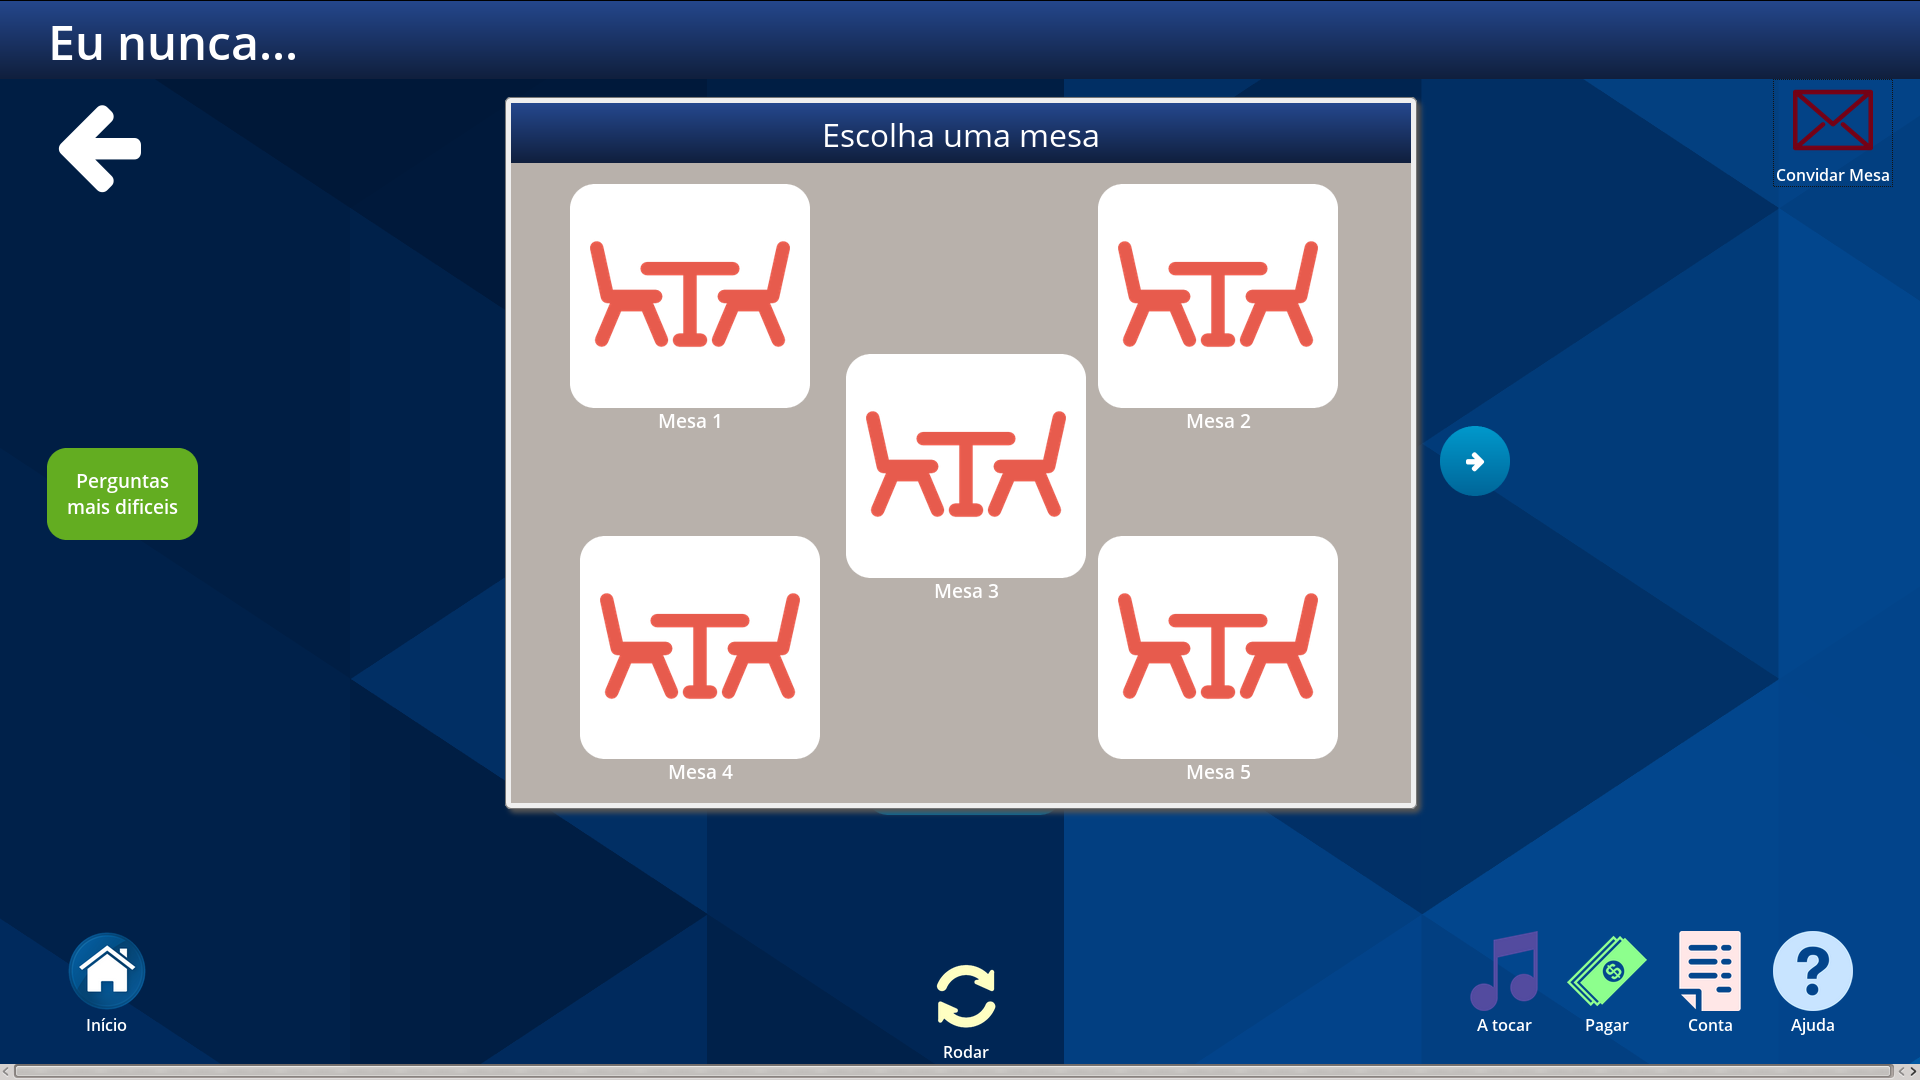
\includegraphics[width=15cm, height=8cm]{user_manual_images/invite_table.png}
De seguida, clicar na mesa com a qual se deseja jogar aparecendo a seguinte mensagem, após o convite ser aceite:\\\\
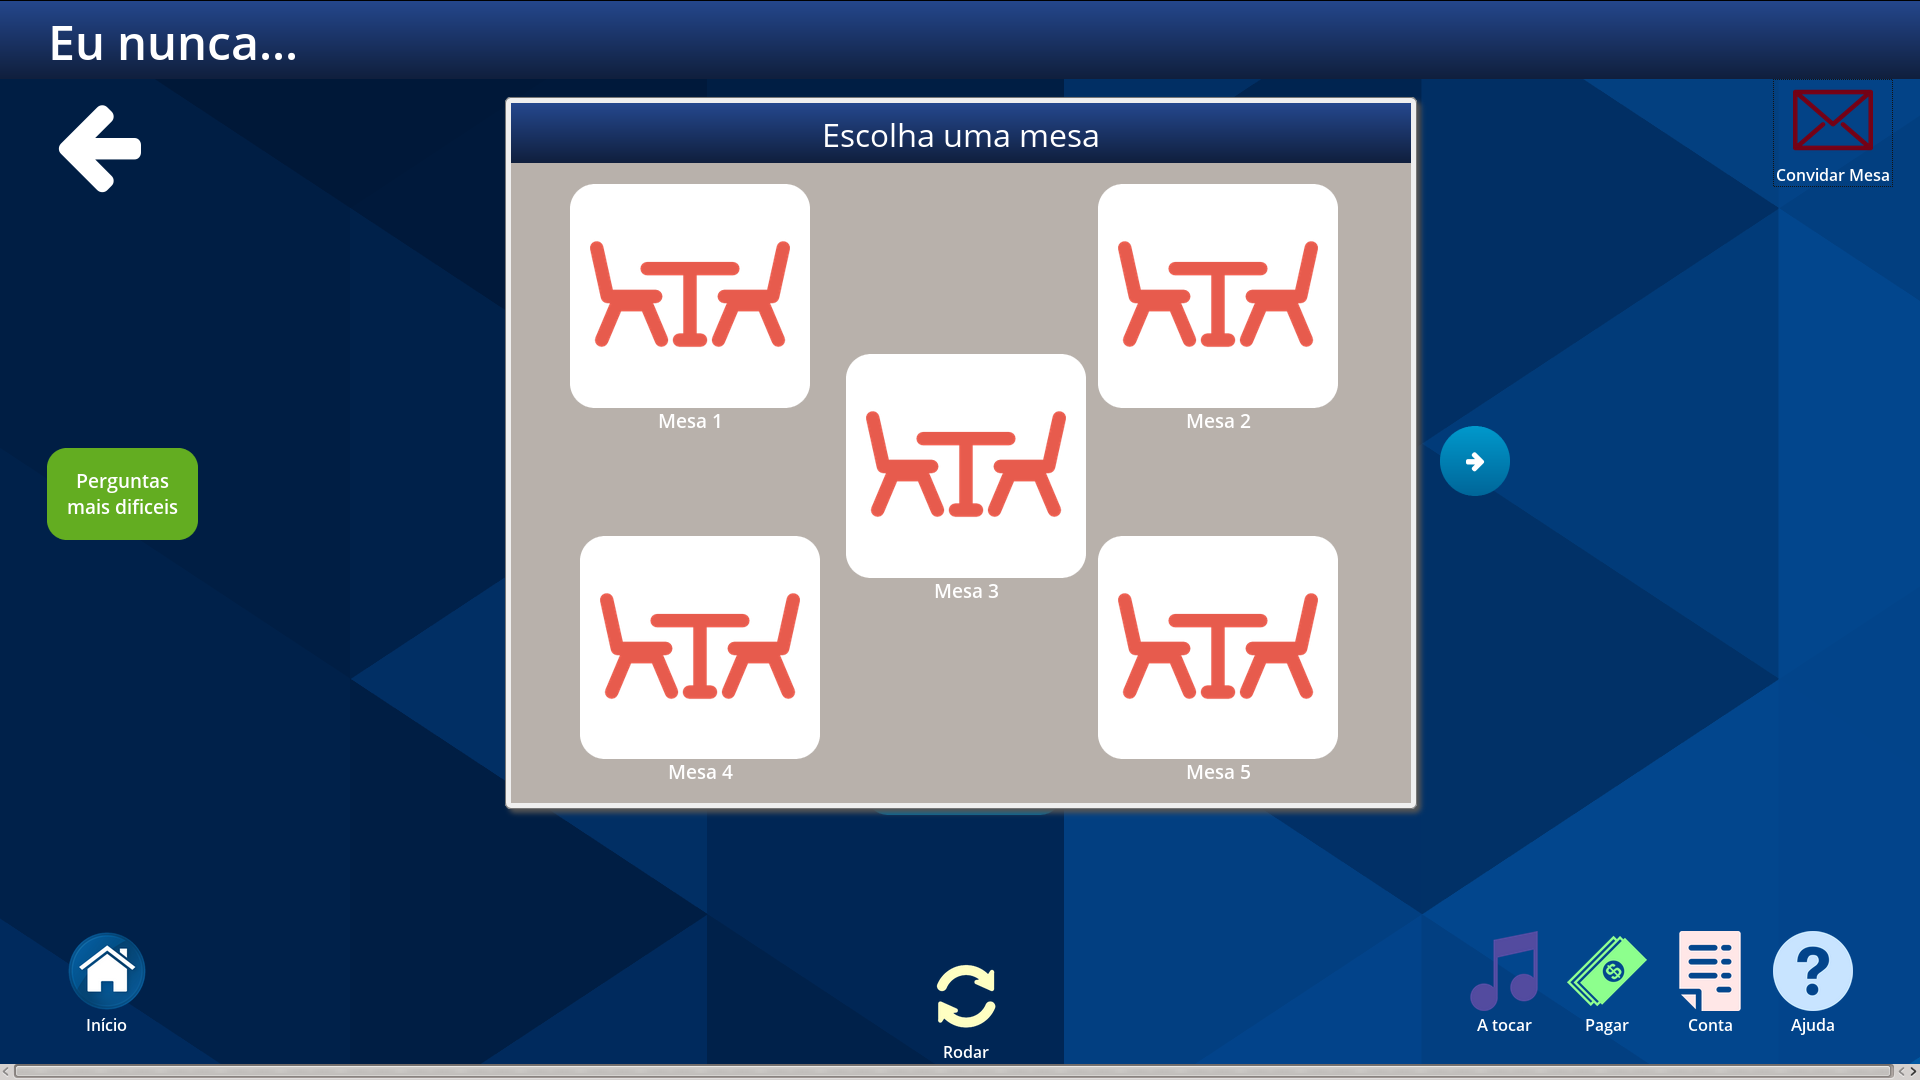
\includegraphics[width=15cm, height=8cm]{user_manual_images/invite_table.png}
\end{document}
